%% Users manual for C++ BOUT code

\documentclass[12pt]{article}
\usepackage[nofoot]{geometry}
\usepackage{graphicx}
\usepackage{fancyhdr}

\usepackage{listings}
\usepackage{color}
\usepackage{textcomp}
\definecolor{listinggray}{gray}{0.9}
\definecolor{lbcolor}{rgb}{0.95,0.95,0.95}
\lstset{
	backgroundcolor=\color{lbcolor},
        language=C++,
	keywordstyle=\bfseries\ttfamily\color[rgb]{0,0,1},
	identifierstyle=\ttfamily,
	commentstyle=\color[rgb]{0.133,0.545,0.133},
	stringstyle=\ttfamily\color[rgb]{0.627,0.126,0.941},
	showstringspaces=false,
	basicstyle=\small,
	numberstyle=\footnotesize,
	numbers=left,
	stepnumber=1,
	numbersep=10pt,
	tabsize=2,
	breaklines=true,
	prebreak = \raisebox{0ex}[0ex][0ex]{\ensuremath{\hookleftarrow}},
	breakatwhitespace=false,
	aboveskip={1.5\baselineskip},
        columns=fixed,
        upquote=true,
        extendedchars=true,
        morekeywords={Field2D,Field3D,Vector2D,Vector3D,real,FieldGroup},
}

%% Modify margins
\addtolength{\oddsidemargin}{-.25in}
\addtolength{\evensidemargin}{-.25in}
\addtolength{\textwidth}{0.5in}
\addtolength{\textheight}{0.25in}
%% SET HEADERS AND FOOTERS

\pagestyle{fancy}
\fancyfoot{}
\renewcommand{\sectionmark}[1]{         % Lower case Section marker style
  \markright{\thesection.\ #1}}
\fancyhead[LE,RO]{\bfseries\thepage}    % Page number (boldface) in left on even
                                        % pages and right on odd pages 
\renewcommand{\headrulewidth}{0.3pt}

\newcommand{\code}[1]{\texttt{#1}}
\newcommand{\file}[1]{\texttt{\bf #1}}

%% commands for boxes with important notes
\newlength{\notewidth}
\addtolength{\notewidth}{\textwidth}
\addtolength{\notewidth}{-3.\parindent}
\newcommand{\note}[1]{
\fbox{
\begin{minipage}{\notewidth}
{\bf NOTE}: #1
\end{minipage}
}}

\newcommand{\pow}{\ensuremath{\wedge} }
\newcommand{\poweq}{\ensuremath{\wedge =} }

\newcommand{\deriv}[2]{\ensuremath{\frac{\partial #1}{\partial #2}}}

\newcommand{\rbtsq}{\ensuremath{\left(RB_\theta\right)^2}}
\newcommand{\sbt}{\ensuremath{\sigma_{B\theta}}}
\newcommand{\apar}{\ensuremath{A_{||}}}
\newcommand{\Bthe}{\ensuremath{B_\theta}}
\newcommand{\Bzeta}{\ensuremath{B_\zeta}}
\newcommand{\hthe}{\ensuremath{h_\theta}}

\begin{document}

\title{BOUT++ Users Manual}
\author{B.Dudson, University of York}
\date{August 7, 2009}
\maketitle

\tableofcontents

\section{Introduction}

BOUT++ is a C++ framework for writing plasma fluid simulations with an arbitrary number of equations
in 3D curvilinear coordinates \cite{Dudson2009,dudson-2008-arxiv}. It has been developed from the original {\bf BOU}ndary {\bf T}urbulence
3D 2-fluid edge simulation code \cite{bout_manual,umansky-2008-bout,xu-2008} written by X.Xu and M.Umansky at LLNL.

Though designed to simulate tokamak edge plasmas, the methods used are very general and almost
any metric tensor can be specified, allowing the code to be used to simulate (for example) plasmas in 
slab, sheared slab, and cylindrical coordinates. The restrictions on the simulation domain
are that the equilibrium must be axisymmetric (in the z coordinate), and that the parallelisation
is done in the $x$ and $y$ (parallel to $\mathbf{B}$) directions.

The aim of BOUT++ is to automate the common tasks needed for simulation codes, and to separate the
complicated (and error-prone) details such as differential geometry, parallel communication, and
file input/output from the user-specified equations to be solved. Thus the equations being solved
are made clear, and can be easily changed with only minimal knowledge of the inner workings of the
code. As far as possible, this allows the user to concentrate on the physics, rather than worrying
about the numerics. This doesn't mean that users don't have to think about numerical methods, and so selecting differencing schemes and boundary conditions is discussed in this manual. The generality of the BOUT++ of course also comes with a limitation: Although there is a large class of problems which can be tackled by this code, there be many more problems which require a more specialised solver and which BOUT++ will not be able to handle. Hopefully this manual will enable you to test whether BOUT++ is suitable for your problem as quickly and painlessly as possible.

This manual is written for the user who wants to run (or modify) existing plasma models, or 
specify a new problem (grid and equations) to be solved. In either case, it's assumed that
the user isn't all that interested in the details of the code.
For a more detailed descriptions of the code internals, see the developer
and reference quides.
After describing how to install BOUT++ (section~\ref{sec:install}) and run a few examples 
(section~\ref{sec:runexamples}, but described in detail in section~\ref{sec:examples}), increasingly sophisticated ways to modify the problem being solved are introduced.
The simplest way to modify a simulation case is by altering the input options, described in
section~\ref{sec:options}. Checking that the options are doing what you think they should be
by looking at the output logs is described in section~\ref{sec:running}, and an overview of the IDL analysis routines
for data post-processing and visualisation is given in section~\ref{sec:output}.
Generating new grid files, particularly for tokamak equilibria, is described in section~\ref{sec:gridgen}.

Up to this point, little programming experience has been assumed, but performing more drastic
alterations to the physics model requires modifying C++ code.
Section~\ref{sec:equations} describes how to write a new physics model specifying the equations to be solved,
using ideal MHD as an example. The remaining sections describe in more detail aspects of using BOUT++:
section~\ref{sec:diffops} describes the differential operators and methods available; section~\ref{sec:staggergrids}
covers the new staggered grid system (which doesn't yet work).

\subsection{License and terms of use}

\begin{verbatim}
Copyright 2010 B.D.Dudson, S.Farley, M.V.Umansky, X.Q.Xu

BOUT++ is free software: you can redistribute it and/or modify
it under the terms of the GNU Lesser General Public License as published by
the Free Software Foundation, either version 3 of the License, or
(at your option) any later version.

BOUT++ is distributed in the hope that it will be useful,
but WITHOUT ANY WARRANTY; without even the implied warranty of
MERCHANTABILITY or FITNESS FOR A PARTICULAR PURPOSE.  See the
GNU Lesser General Public License for more details.

You should have received a copy of the GNU Lesser General Public License
along with BOUT++.  If not, see <http://www.gnu.org/licenses/>.

A copy of the LGPL license is in COPYING.LESSER. Since this is based
on (and refers to) the GPL, this is included in COPYING.
\end{verbatim}

BOUT++ is free software, but since it is a
scientific code we also ask that you show professional courtesy
when using this code:

\begin{enumerate}
\item Since you are benefiting from work on BOUT++, we ask that you
  submit any improvements you make to the code to us by emailing 
  Ben Dudson at bd512@york.ac.uk
\item If you use BOUT++ results in a paper or professional publication,
  we ask that you send your results to one of the BOUT++ authors
  first so that we can check them. It is understood that in most cases
  if one or more of the BOUT++ team are involved in preparing results
  then they should appear as co-authors.
\item Publications or figures made with the BOUT++ code should acknowledge the
  BOUT++ code by citing B.Dudson et. al. Comp.Phys.Comm 2009 \cite{Dudson2009}
  and/or other BOUT++ papers. See the file CITATION for details.
\end{enumerate}

\section{Starting}

This section describes how to install and start using BOUT++. At the time of
writing, the latest version of the code can be obtained from the NERSC
subversion repository:
\begin{verbatim}
svn co svn+ssh://user@svn.nersc.gov/svn/bout/trunk
\end{verbatim}

However you obtain the distribution, there should be several subdirectories,
currently \file{BOUT++}, \file{idllib}, and \file{tokamak\_grids}. A description
of each directory is given in the README file.

Once you have checked out a branch, the core BOUT++ code is in the
\file{BOUT++} directory (with source in \file{BOUT++/SRC}), and
section~\ref{sec:install} describes how to compile this as a library which
can then be used by many different fluid models. Some example models and test
problems are in the \file{BOUT++/examples} directory and are described in
section~\ref{sec:examples}.

\subsection{Documentation}

Various sources of documentation are:
\begin{itemize}
\item Most directories in the BOUT++ distribution contain a README file. This should
describe briefly what the contents of the directory are and how to use them.
\item This users' manual, which goes through BOUT++ from a users's point of view
\item The developer's manual, which gives details of the internal working of the code.
\item The reference guide, which summarises functions, settings etc. Intended more for
quick reference rather than a guide.
\item The \file{elm\_reduced} manual describes in great detail running ELM simulations with BOUT++,
and derivations of the model used.
\item Most of the code contains Doxygen comment tags (which are slowly getting better). 
Running doxygen (\file{www.doxygen.org}) on these files should therefore generate an HTML
reference. This is probably going to be the most up-to-date documentation.
\end{itemize}

\subsection{Installation}
\label{sec:install}

BOUT++ uses several external libraries, and unless these are already installed, you will need to install them yourself. 

BOUT++ can currently use two different file formats: Portable Data Binary
(PDB) which is part of PACT\footnote{\code{http://pact.llnl.gov}}, and
NetCDF-4\footnote{\code{http://www.unidata.ucar.edu/software/netcdf/}}.
PDB was developed at LLNL, was used in the UEDGE and BOUT codes, and 
was the original format used by BOUT++. NetCDF is a more widely used
format and so has many more tools for viewing and manipulating files.
In particular, the NetCDF-4 library can produce files in either
NetCDF3 ``classic'' format, which is backwards-compatible with NetCDF
libraries since 1992, or in the newer NetCDF4 format, which is based
on (and compatible with) HDF5. If you have both libraries installed then
BOUT++ can use both simultaneously, for example reading in grid files in PDB
format, but writing output data in NetCDF format.

\subsubsection{Libraries}

On most large systems (e.g. Franklin, HECToR etc.) you will not be able to install
libraries into system directories. This is a run-through of how to install the required libraries
on Franklin, but the same steps should work on most systems.

BOUT++ can use the following libraries:
\begin{itemize}
  \item MPI (Message Passing Interface) {\bf [Required]}. Should work with most implementations, though mostly tested with MPICH.
  \item FFTW-3 (Fastest Fourier Transform  in the West) {\bf [Required]} \code{http://www.fftw.org/} 
  \item NetCDF-4 
  \item PACT \code{http://pact.llnl.gov/} for reading and writing Portable Data Binary (PDB) format files. This is mainly for backwards compatibility with BOUT and UEDGE, and NetCDF-4 is recommended.
  \item SUNDIALS \code{https://computation.llnl.gov/casc/sundials/main.html}
  \item LAPACK for linear solvers
\end{itemize}

A bare minimum to get BOUT++ running is an MPI implementation (e.g. MPICH, OpenMPI, LAM), FFTW-3, and one (or both) of NetCDF or PACT. 
To install these libraries in your home directory,  first create a directory ``install'' which is
going to be used for temporary installation files,  and a directory ``local'' where the libraries are going to be installed:
\begin{verbatim}
 ~/ $ mkdir install
 ~/ $ mkdir local
 ~/ $ mkdir local/bin
 ~/ $ mkdir local/lib
\end{verbatim}

Then add your local directories to environment variables. For BASH shells:
\begin{verbatim}
 ~/ $ export PATH=$HOME/local/bin:$PATH
 ~/ $ export LD_LIBRARY_PATH=$HOME/local/lib:$LD_LIBRARY_PATH
\end{verbatim}
or for CSH type shells:
\begin{verbatim}
 ~/ $ setenv PATH $HOME/local/bin:$PATH
 ~/ $ setenv LD_LIBRARY_PATH $HOME/local/lib:$LD_LIBRARY_PATH
\end{verbatim}
These two lines should be added to the end of your login scripts (e.g. \file{~/.profile})

Then download the NetCDF, FFTW, SUNDIALS and (optionally) PACT libraries, and put them into ``install''. This
tutorial is with the following versions:
\begin{verbatim}
 ~/ $ ls install
fftw-3.2.1.tar.gz    pact-2.1.0.tar.gz
netcdf-4.0.1.tar.gz  sundials-2.4.0.tar.gz
\end{verbatim}

Before installing, make sure the correct version of \file{install} is being used by running
\begin{verbatim}
 ~/ $ which install
\end{verbatim}
This should point to a system directory like \file{/usr/bin/install}. Sometimes when IDL has been
installed, this points to the IDL install (e.g. something like \file{/usr/common/usg/idl/idl70/bin/install} on Franklin). A quick way to fix this is to create a link from your local bin to the system install:\begin{verbatim}
 ~/ $ ln -s /usr/bin/install $HOME/local/bin/
\end{verbatim}
``which install'' should now print the install in your local bin directory.

Most of these libraries can be installed by unzipping the archive, configuring and making. For example, the NetCDF library can be built using:
\begin{verbatim}
~/install/ $ tar -xzvf netcdf-4.0.1.tar.gz
~/install/ $ cd netcdf-4.0.1
~/install/netcdf-4.0.1/ $ ./configure --prefix=$HOME/local
~/install/netcdf-4.0.1/ $ gmake
~/install/netcdf-4.0.1/ $ gmake install
\end{verbatim}

NOTES: 
\begin{itemize}
\item If you want to output to HDF5 then you need to first install
  the zlib and HDF5 libraries, and then compile NetCDF with HDF5 support.
\begin{verbatim}
~/install/netcdf-4.0.1/ $ ./configure --prefix=$HOME/local
\end{verbatim}
\item On Franklin, SUNDIALS needs to be compiled with ``--with-mpicc=cc'' to
  force it to build the parallel libraries
\end{itemize}

Details on installing PACT are given in Appendix~\ref{apx:pact}. NOTE: This
can be a giant hassle, and is only really needed
for backwards compatibility with BOUT. If you're not interested in using PDB files
you can skip this.

The SUNDIALS library needs to have MPI enabled, so after configuring, check the output and look for something like this:
\begin{verbatim}
MPI-C Settings
--------------

checking if using MPI-C script... yes
checking if absolute path to mpicc was given... no
checking for mpicc... none
configure: WARNING: cannot find MPI-C compiler
\end{verbatim}

If you see this warning, you need to tell CVODE which MPI compiler to use. This happens
on machines where the MPI compilers are given non-standard names. For IBM AIX machines,
use
\begin{verbatim}
$ ./configure --prefix=$HOME/local/ --with-mpicc=xlC
\end{verbatim}

\subsubsection{BOUT++}

Once you have the libraries installed, you can install BOUT++.
In the root directory of the BOUT++ distribution is a file \file{INSTALL} 
which will contain more details on installation, including troubleshooting.
For most systems however the installation should consist of running the
following commands in the BOUT++ root directory:
\begin{verbatim}
./configure
gmake
\end{verbatim}
This should detect the setting needed automatically. The main things it's
looking for are
\begin{itemize}
\item NetCDF installation. When NetCDF is installed, a script \file{nc-config}
should be put into somewhere on the path. If this is found then configure
should have all the settings it needs. If this isn't found then configure
will search for the NetCDF include and library files. To specify the location
of these files, use
\begin{verbatim}
    ./configure --with-netcdf=/path/to/netcdf/
\end{verbatim}
\item A PACT installation (\file{http://pact.llnl.gov}) for PDB file I/O. One of the places configure
  will look is in your home/local directory. If you do not want PDB support, configure with
\begin{verbatim}
    ./configure --with-pdb=no
\end{verbatim}
If you do this, you will need to enable NetCDF support (see below).
If you ignored the earlier instructions and installed PACT into a non-standard location, you can specify this using
\begin{verbatim}
    ./configure PACT=/path/to/pact/
\end{verbatim}
\item MPI C and C++ compilers. These are usually called something like mpicc and mpiCC (or mpicxx), but if your compilers aren't recognised then set them using
\begin{verbatim}
     ./configure MPICC=<your C compiler> MPICXX=<your C++ compiler>
\end{verbatim}
\end{itemize}

When the compilation finishes the BOUT++ library should be in \file{lib/libbout++.a}.
If you have trouble compiling see the \file{INSTALL} file for more details.

To enable NetCDF support, you will need to install NetCDF version 4.0.1 or later. 
Note that although the NetCDF-4 library is used for the C++ interface, by default
BOUT++ writes the ``classic'' format, which can be read by any NetCDF installation
since 1994 (version 2.3). Because of this, you don't need to install zlib or HDF5
for BOUT++ NetCDF support to work.

To enable NetCDF support,
\begin{verbatim}
./configure --with-netcdf
\end{verbatim}
or
\begin{verbatim}
./configure --with-netcdf=/path/to/netcdf/
\end{verbatim}

NOTES:
\begin{itemize}
\item On LLNL's Grendel, mpicxx is broken. Use mpiCC instead by passing ``MPICXX=mpiCC'' to configure. Also need to specify this to NetCDF library by passing ``CXX=mpiCC'' to NetCDF configure.
\end{itemize}

\subsubsection{Solver library}

As of July 2010, BOUT++ can be compiled with several solver libraries, and the desired one
selected at runtime (thanks to factory magic by S.Farley).

The BOUT++ distribution used to include a 1998 version of CVODE by Scott D. Cohen and Alan C.
Hindmarsh, which was the default time integration solver. This is the easiest to install, and
can be downloaded and compiled automatically by using the option
\begin{verbatim}
   ./configure --download-pvode
\end{verbatim}
Whilst no serious bugs have been found in this code
(as far as I am aware), several features such as user-supplied preconditioners and constraints cannot
be used with this solver. Currently, BOUT++ also supports the SUNDIALS solvers CVODE and
IDA\footnote{available from \code{https://computation.llnl.gov/casc/sundials/main.html}}.

The modern SUNDIALS CVODE solver is essentially the same as the 1998 CVODE (with some tweaking,
re-arranging etc.), but this solver allows users to supply their own preconditioner 
and Jacobian functions. To use this solver, use
\begin{verbatim}
./configure --with-cvode
\end{verbatim}
or
\begin{verbatim}
./configure --with-cvode=/path/to/cvode/
\end{verbatim}
if your CVODE library is in a non-standard place.

The SUNDIALS IDA solver is a Differential-Algebraic Equation (DAE) solver, which evolves a system of the form
$\mathbf{f}\left(\mathbf{u}, \dot\mathbf{u}, t\right) = 0$. This allows algebraic constraints on variables
to be specified. If you want this functionality, compile in the IDA library using
\begin{verbatim}
./configure --with-ida
\end{verbatim}
or
\begin{verbatim}
./configure --with-ida=/path/to/ida/
\end{verbatim}

\subsubsection{PETSc}

BOUT++ can use PETSc for time-integration:
\begin{verbatim}
./configure --with-petsc
\end{verbatim}

This will allow use of a greater number of sophisticated time-integration
packages and preconditioning methods, and is under development.

\subsubsection{FFT library}

BOUT++ needs the the FFTW-3 (Fastest Fourier Transform in the West)
library\footnote{\code{http://www.fftw.org/}}. The configure script will
search for an installation, but if you've installed it in a strange place then
specify the path to the installation:
\begin{verbatim}
./configure --with-fftw=/path/to/fftw/
\end{verbatim}

\subsubsection{LAPACK}

As with FFT routines, the TRUNK branch does contain fall-back routines
for solving tri- and band-diagonal complex and real matrices. These
are however descended from Numerical Recipes code, and so are removed
from RELEASE.

To replace these routines, BOUT++ can use the LAPACK library. This is
written in FORTRAN 77, which can cause linking headaches.
To enable these routines in TRUNK (always enabled in RELEASE), use
\begin{verbatim}
./configure --with-lapack
\end{verbatim}
and to specify a non-standard path
\begin{verbatim}
./configure --with-lapack=/path/to/lapack
\end{verbatim}

\subsection{Running the examples}
\label{sec:runexamples}

To use the BOUT++ library, set an environment variable {\bf BOUT\_TOP} to point to the BOUT++ root
directory (the directory containing make.config and configure). Actually this is not strictly true since
you can compile the examples by just running
\begin{verbatim}
gmake examples
\end{verbatim}
in the BOUT++ root directory, but setting {\bf BOUT\_TOP} lets you compile examples in different
directories, and makes it easier to develop cases.

The \file{examples/} directory contains some test cases for a variety of fluid models. In many cases
there are two scripts for running and then an IDL script to plot the results:
\begin{verbatim}
./runcase.sh
idl runidl.pro
\end{verbatim}

Assuming these examples work (which they should), looking through the scripts and code
may give you an idea of how BOUT++ works. More information on setting up and running BOUT++ is given
in section~\ref{sec:running}, and details of analysing the results using IDL are given in
section~\ref{sec:output}.

\subsection{When things go wrong}

BOUT++ is still under development, and so occasionally you may be lucky
enough to discover a new bug. This is particularly likely if you're modifying
the physics module source code (see section~\ref{sec:equations}) when you
need a way to debug your code too.

\begin{itemize}
\item Check the end of each processor's log file (tail data/BOUT.log.*). When BOUT++ exits before
it should, what is printed to screen is just the output from processor 0.
If an error occurred on another processor then the error message will be written to it's log file instead.
\item By default when an error occurs a kind of stack trace is printed which shows which functions
were being run (most recent first). This should give a good indication of where an error occured.
If this stack isn't printed, make sure checking is set to level 2 or higher (./configure --with-checks=2)
\item If the error is a segmentation fault, you can try a debugger such as totalview
\item If the error is due to non-finite numbers, increase the checking level
(./configure --with-checks=3) to perform more checking of values
and (hopefully) find an error as soon as possible after it occurs.
\end{itemize}

\section{BOUT++ options}
\label{sec:options}

The inputs to BOUT++ are a binary grid file in NetCDF or PDB format,
and a text file with options. Generating input grids for tokamaks is
described in section~\ref{sec:gridgen}. The grid file describes the size
and topology of the X-Y domain, metric tensor components and usually
some initial profiles. The option file specifies the size of the domain
in the symmetric direction (Z), and controls how the equations are evolved
e.g. differencing schemes to use, and boundary conditions.
In most situations, the grid file will be used in many different simulations,
but the options may be changed frequently. 

The input file \file{BOUT.inp} includes comments and should be fairly
self-explanatory. The format is the same as a windows INI file, consisting
of \code{name = value} pairs. Comments are started
with a semi-colon, which comments out the rest of the line. Values can be:
\begin{itemize}
\item Integers
\item Real values
\item Booleans
\item Strings
\end{itemize}
Options are also divided into sections, which start with the section name in square brackets.
\begin{verbatim}
[section1]

something = 132         ; an integer
another = 5.131         ; a real value
yetanother = true       ; a boolean
finally = "some text"   ; a string
\end{verbatim}
\note{Options are NOT case-sensitive: \code{TwistShift} and \code{twistshift} are the same variable}

Have a look through the examples to see how the options are used.

\subsection{General options}

At the top of the BOUT.inp file (before any section headers), 
options which affect the core code are listed. 
These are common to all physics models, and the most useful of them are:
\begin{verbatim}
NOUT = 100       # number of time-points output
TIMESTEP = 1.0   # time between outputs
\end{verbatim}
which set the number of outputs, and the time step between them. Note that
this has nothing to do with the internal timestep used to advance the
equations, which is adjusted automatically. What time-step to use depends
on many factors, but for high-$\beta$ reduced MHD
ELM simulations reasonable choices are \code{1.0}
for the first part of a run (to handle initial transients), then around \code{10.0} for the
linear phase. Once non-linear effects become important, you will have to reduce the timestep to
around \code{0.1}.

Most large clusters or supercomputers have a limit on how long a job can
run for called ``wall time'', because it's the time taken according to a
clock on the wall, as opposed to the CPU time actually used.
If this is the case, you can use the option
\begin{verbatim}
wall_limit = 10 # wall clock limit (in hours)
\end{verbatim}
BOUT++ will then try to quit cleanly before this time runs out. Setting a
negative value (default is -1) means no limit.

Often it's useful to be able to restart a simulation from a chosen point,
either to reproduce a previous run, or to modify the settings and re-run.
A restart file is output every timestep, but this is overwritten each time,
and so the simulation can only be continued from the end of the last
simulation. Whilst it is possible to create a restart file from the output
data afterwards, it's much easier if you have the restart files. Using the
option
\begin{verbatim}
archive = 20
\end{verbatim}
saves a copy of the restart files every 20 timesteps, which can then be used as a starting point.

The X and Y size of the computational grid is set by the grid file, but the
number of points in the Z (axisymmetric) direction is specified in the options
file:
\begin{verbatim}
MZ = 33
\end{verbatim}
This must be $\texttt{MZ} = 2^n + 1$, and can be $2,3,5,9,\ldots$. The power of 2 is so
that FFTs can be used in this direction; the $+1$ is for historical reasons (inherited from BOUT)
and is going to be removed at some point.

Since the Z dimension is periodic, the domain size is specified as multiples or fractions of $2\pi$.
To specify a fraction of $2\pi$, use
\begin{verbatim}
ZPERIOD = 10
\end{verbatim}
This specifies a Z range from $0$ to $2\pi / \code{ZPERIOD}$, and is useful for simulation
of tokamaks to make sure that the domain is an integer fraction of a torus. If instead you want
to specify the Z range directly (for example if Z is not an angle), there are the options
\begin{verbatim}
ZMIN = 0.0
ZMAX = 0.1
\end{verbatim}
which specify the range in multiples of $2\pi$.

\note{For users of BOUT, the definition of \code{ZMIN} and \code{ZMAX} has been changed.
These are now fractions of $2\pi$ radians i.e. $\code{dz} = 2\pi(\code{ZMAX - ZMIN})/\code{(MZ-1)}$}

In BOUT++, grids can be split between processors in both X and Y directions. By
default only Y decomposition is used, and to use X decomposition you must specify
the number of processors in the X direction:
\begin{verbatim}
NXPE = 1  # Set number of X processors
\end{verbatim}

The grid file to use is specified relative to the root directory where the simulation
is run (i.e. running ``\code{ls ./data/BOUT.inp}'' gives the options file)
\begin{verbatim}
grid = "data/cbm18_8_y064_x260.pdb"
\end{verbatim}

\subsection{Solver options}

There are a number of options which affect the core BOUT++ code
such as choice of differencing methods. These are divided into sections:
differencing, Laplacian inversion, communications, and CVODE solver.

\begin{itemize}
\item Differencing methods are specified in three section (\code{[ddx]}, \code{[ddy]} and \code{[ddz]}), one
  for each dimension. 
  \begin{itemize}
  \item \code{first}, the method used for first derivatives
  \item \code{second}, method for second derivatives
  \item \code{upwind}, method for upwinding terms
  \end{itemize}
  The methods which can be specified are U1, U4, C2, C4, W2, W3, FFT
  Apart from FFT, the first letter gives the type of method (U = upwind, C = central, W = WENO), and the number gives
  the order.
\item The main solver settings are the absolute and relative solver tolerances, \code{ATOL} and \code{RTOL}.
  In addition there are \code{mudq} and \code{mldq}, \code{mukeep} and \code{mlkeep}.
\item The communication system has a section \code{[comms]}, with a true/false option \code{async}. This
  determines whether asyncronous MPI sends are used; which method is faster varies (though not by much)
  with machine and problem.
\end{itemize}

\subsection{Model-specific options}

The options which affect a specific physics model vary, since they are defined in the physics module itself
(see section~\ref{sec:inputopts}). They should have a separate section, for example the high-$\beta$
reduced MHD code uses options in a section called \code{[highbeta]}.

There are three places to look for these options: the BOUT.inp file; the physics model C++ code, and 
the output logs. The physics module author should ideally have an example input file, with commented options
explaining what they do; alternately they may have put comments in the C++ code for the module. 
Another way is to look at the output logs: when BOUT++ is run, (nearly) all options used are printed 
out with their default values. This won't provide much explanation of what they do, but may be useful anyway.
See section~\ref{sec:output} for more details.

\subsection{Variable initialisation}

Each variable being evolved has its own section, with the same name as the
output data. For example, the high-$\beta$ model has variables ``P'',
``jpar'', and ``U'', and so has sections \code{[P]}, \code{[jpar]},
\code{[U]} (not case sensitive). 

The shape of the initial value is specified for each dimension separately
using the options \code{xs\_opt}, \code{ys\_opt}, and \code{zs\_opt}. These
are set to an integer: 
\begin{enumerate}
\setcounter{enumi}{-1}
\item Constant (this is the default)
\item Gaussian, with a peak location given by \code{xs\_s0}, \code{ys\_s0},
  \code{zs\_s0} as a fraction of the domain (i.e. $0 \rightarrow 1$.
  The width is given by \code{*s\_wd}, also as a fraction of the domain size.
\item Sinusoidal, with the number of periods given by \code{*s\_mode}. 
\item Mix of mode numbers, with psuedo-random phases.
\end{enumerate}
The magnitude of the initial value is given by the variable \code{scale}.

Defaults for all variables can be set in a section called \code{[All]},
so for example the options below:
\begin{verbatim}
[All]
scale = 0.0 # By default set variables to zero

xs_opt = 1  # Gaussian in X
ys_opt = 1  # Gaussian in Y
zs_opt = 2  # Sinusoidal in Z (axisymmetric direction)

xs_s0 = 0.5 # Peak in the middle of the X direction 
xs_wd = 0.1 # Width is 10% of the domain 

ys_s0 = 0.5 # Peak in the middle of the Y direction
ys_wd = 0.3 # Width is 30% of the Y domain

zs_mode = 3 # 3 periods in the Z direction

[U]
scale = 1.0e-5  # Amplitude for the U variable, overrides default
\end{verbatim}

For field-aligned tokamak simulations, the Y direction is along the
field and in the core this will have a discontinuity at the twist-shift
location where field-lines are matched onto each other. To handle this,
a truncated Ballooning transformation can be used to construct a smooth
initial perturbation:
\[
U_0^{balloon} = \sum_{i=-N}^N F\left(x\right)G\left(y + 2\pi i\right)H\left(z + q2\pi i\right)
\]

\note{The initial profiles code currently doesn't work very well for grids with branch-cuts (e.g. divertor tokamak), and will often have jumps which then make timesteps smaller}

\subsection{Boundary conditions}

Like the variable initialisation, boundary conditions can be set for
each variable in individual sections, with default values in a section
\code{[All]}. Boundary conditions are specified for each variable, being 
applied to variable itself during initialisation, and the time-derivatives
at each timestep.

When finding the boundary condition for a variable \code{var} on a boundary region, 
the options are checked in order from most to least specific:
\begin{itemize}
\item Section \code{var}, \code{bndry\_} + region name. Depending on the mesh file, regions
  of the grid are given labels. Currently
  these are \code{core}, \code{sol}, \code{pf} and \code{target} which
  are intended for tokamak edge simulations. Hence the variables checked
  are \code{bndry\_core}, \code{bndry\_pf} etc.
\item Section \code{var}, \code{bndry\_} + boundary side. These names are
  \code{xin}, \code{xout}, \code{yup} and \code{ydown}. 
\item Section \code{var}, variable \code{bndry\_all}
\item The same settings again except in section \code{All}.
\end{itemize}
The most general setting is therefore \code{bndry\_all} in the \code{All} 
section.

Boundary conditions are given names and currently include:
\begin{itemize}
\item \code{dirichlet} - Set to zero
\item \code{neumann} - Zero gradient
\item \code{zerolaplace} - Laplacian = 0, decaying solution (X boundaries only)
\item \code{constlaplace} - Laplacian = const, decaying solution (X boundaries only)
\end{itemize}
The zero- or constant-Laplacian boundary conditions works as follows:
\begin{eqnarray*}
\nabla_\perp^2 f &=& 0 \\
&\simeq& g^{xx}\frac{\partial^2 f}{\partial x^2} + g^{zz}\frac{\partial^2 f}{\partial z^2}
\end{eqnarray*}
which when Fourier transformed in $z$ becomes: 
\[
g^{xx}\frac{\partial^2 \hat{f}}{\partial x^2} - g^{zz}k_z^2 \hat{f} = 0
\]
which has the solution
\[
\hat{f} = Ae^{xk_z\sqrt{g^{zz}/g^{xx}}} + Be^{-xk_z\sqrt{g^{zz}/g^{xx}}}
\]
Assuming that the solution should decay away from the domain, on the inner
$x$ boundary $B = 0$, and on the outer boundary $A = 0$. 

\subsection{Relaxing boundaries}

All boundaries can be modified to be ``relaxing'' which are a combination
of zero-gradient time-derivative, and whatever boundary condition they are
applied to. The idea is that this prevents sharp discontinuities at boundaries
during transients, whilst maintaining the desired boundary condition on
longer timescales. In some cases this can improve the numerical stability
and timestep.

For example, \code{relax(dirichlet)} will make a field $f$ at point $i$ in the
boundary follow a point $i-1$ in the domain:
\[
\left.\deriv{f}{t}\right|_i = \left.\deriv{f}{t}\right|_{i-1}  - f_i / \tau
\]
where $\tau$ is a timescale for the boundary (currently set to 0.1, but will
be a global option). S
When the time-derivatives are slow close to the boundary, the boundary
relaxes to the desired condition (Dirichlet in this case), but when the
time-derivatives are large then the boundary approaches Neumann to reduce
discontinuities.

\section{Running BOUT++}
\label{sec:running}

The command to run a parallel code varies between machines, but on most small clusters
the following command should work:
\begin{verbatim}
mpirun -np <num. proc> <command>
\end{verbatim}
so to run the \code{highbeta\_reduced} case on 4 processors:
\begin{verbatim}
cd <path>/BOUT++/examples/highbeta_elm/
mpirun -np 4 ./highbeta_reduced
\end{verbatim}

\subsection{Startup output}

When BOUT++ is run, it produces a lot of output initially, mainly listing
the options which have been used so you can check that it's doing what you
think it should be. It's generally a good idea to scan over this
see if there are any important warnings or errors. Each processor outputs
its own log file \file{BOUT.log.\#}
and the log from processor 0 is also sent to the screen. This output may
look a little different if it's out of date, but the general layout will
probably be the same.

First comes the introductory blurb:
\begin{verbatim}
BOUT++ version 0.70
MD5 checksum: 9703e3588ef9e66cc89a893e4706d8ac
Code compiled on Aug  8 2009 at 14:21:26
B.Dudson (University of York), M.Umansky (LLNL) 2007
Based on BOUT by Xueqiao Xu, 1999

Compile-time options:
        Checking enabled, level 2
        Signal handling enabled
        PDB support enabled
        netCDF support disabled

Run started at  : Sat Aug  8 14:22:58 2009

Processor number: 0 of 4
\end{verbatim}
The version number (0.70 here) gets increased occasionally after some major feature has been added.
To help match simulations to code versions, there's also the timestamps when the core BOUT++ code
was compiled and when the run was started. This helps work out later if a given feature or bug-fix
was implemented when a simulation was run. When compiled, the core
part of BOUT++ calculates an MD5 checksum of all its code. This makes it
possible to verify precisely which version of the code was used for any given
run.

Then comes those options which affect the core BOUT++ code:
\begin{verbatim}
Reading options file data/BOUT.inp
	Option NOUT = 50
	Option TIMESTEP = 1.000000e+02
	Option WALL_LIMIT = -1.000000e+00 (default)
Archiving restart files every 20 iterations
	Option dump_float = true (default)
	Option ShiftXderivs = false
	Option IncIntShear = false (default)
	Option ShiftInitial = false (default)
	Option TwistShift = false
	Option ShiftOrder = 0 (default)
	Option TwistOrder = 0 (default)
	Option non_uniform = false (default)
	Option MZ = 65
	Option zperiod = 1 (default)
	Option ZMIN = 0.000000e+00
	Option ZMAX = 2.850500e-03
	Option MXG = 2
	Option MYG = 2
	Option BoundaryOnCell = false (default)
	Option StaggerGrids = false (default)
	Option NXPE = 1 (default)
\end{verbatim}
This lists each option and the value it has been assigned.
Anything not specified in the input
file is given its default value and has \code{(default)} after it.

\begin{verbatim}
Applying Twist-Shift condition. Interpolation: FFT
\end{verbatim}
Matching twisting flux-tubes back onto themselves requires some form of interpolation. 
This should always be set to FFT.

\begin{verbatim}
Using shifted X derivatives. Interpolation: FFT
\end{verbatim}
To get radial derivatives, the quasi-ballooning coordinate method is used (see
section~\ref{sec:shiftcoords}). The upshot of this is that to get radial derivatives,
interpolation in Z is needed. This should also always be set to FFT.

\begin{verbatim}
Setting X differencing methods
        First       :  Fourth order central (C4)
        Second      :  Fourth order central (C4)
        Upwind      :  Third order WENO (W3)
Setting Y differencing methods
        First       :  Fourth order central (C4)
        Second      :  Fourth order central (C4)
        Upwind      :  Third order WENO (W3)
Setting Z differencing methods
        First       :  Fourth order central (C4)
        Second      :  Fourth order central (C4)
        Upwind      :  Third order WENO (W3)
\end{verbatim}

This is a list of the differential methods for each direction. These are set in the 
BOUT.inp file (\code{[ddx]}, \code{[ddy]} and \code{[ddz]} sections), but can be overridden
for individual operators. In brackets are the code used to specify the method in BOUT.inp.

At this point, BOUT++ reads the grid file, and works out the topology of the grid,
and connections between processors.
\begin{verbatim}
Setting grid format
	File extension not recognised for 'data/uedge.grd.pdb_slab.6b5.r1'
Grid: Reading file 'cbm18_8_y064_x260.pdb'
	WARNING: Number of inner y points 'ny_inner' not found. Setting to 32
	EQUILIBRIUM IS SINGLE NULL (SND) 
	Option xperiodic = false (default)
Connection between top of Y processor 3 and bottom of 0 in range 0 <= x < 260
=> This processor sending in down
WARNING adding connection: poloidal index -1 out of range
\end{verbatim}

Optional quantities (such as \code{ny\_inner} in this case) which
are not specified are given a default (best-guess) value, and a warning is printed.


\begin{verbatim}
        MYPE_IN_CORE = 1
        DXS = 260, DIN = 3. DOUT = -1
        UXS = 0, UIN = -1. UOUT = 1
        XIN = -1, XOUT = -1
        Twist-shift: DI 
\end{verbatim}

BOUT++ then tries to read the metric coefficients from the grid file:
\begin{verbatim}
        WARNING: Metric coefficient 'g11' not found
        WARNING: Metric coefficient 'g22' not found
        WARNING: Metric coefficient 'g33' not found
        WARNING: Metric coefficient 'g12' not found
        WARNING: Metric coefficient 'g13' not found
        WARNING: Metric coefficient 'g23' not found
\end{verbatim}
These warnings are printed because the coefficients have not been specified in the 
grid file, and so the metric tensor is set to the default identity matrix.

\begin{verbatim}
Calculating differential geometry terms
        Maximum error in diagonal inversion is 0.000000e+00
        Maximum error in off-diagonal inversion is 0.000000e+00
\end{verbatim}
If only the contravariant components (\code{g11} etc.) of the metric tensor are specified,
the covariant components (\code{g\_11} etc.) are calculated by inverting the metric tensor matrix. 
Error estimates are then calculated by calculating $g_{ij}g^{jk}$ as a check.
Since no metrics were specified in the input, the metric tensor was set to the identity
matrix, making inversion easy and the error tiny.
\begin{verbatim}
       	WARNING: Could not read 'J' from grid. Setting to zero
        WARNING: Jacobian 'J' not found. Calculating from metric tensor
       	Maximum difference in Bxy is 2.120668e+00
       	Communicating connection terms
       	Option comms / async = false
        Option comms / pre_post = false (default)
       	done
\end{verbatim}

\begin{verbatim}
Setting file formats
        Using PDB format for file 'data/BOUT.dmp.0.pdb'
        Using PDB format for file 'data/BOUT.restart.0.pdb'
\end{verbatim}

The laplacian inversion code is initialised, and prints out the options used.
\begin{verbatim}
Initialising Laplacian inversion routines
       	Option comms / async = false
       	Option laplace / filter = 2.000000e-01 (default)
       	Option laplace / low_mem = false (default)
       	Option laplace / use_pdd = false (default)
       	Option laplace / all_terms = false (default)
       	Using serial algorithm
       	Option laplace / max_mode = 26 (default)
\end{verbatim}

After this comes the physics module-specific output:
\begin{verbatim}
Initialising physics module
        .
        .
        .
\end{verbatim}
This typically lists the options used, and useful/important normalisation factors etc.
See the \file{elm\_reduced} manual for an explanation of the output from the
high-$\beta$ reduced MHD model.

If BOUT++ is being restarted from a previous point, the restart file is read, 
and the time printed:
\begin{verbatim}
Datafile: Reading file 'data/BOUT.restart.0.pdb'
Restarting at iteration 200, simulation time 1.100000e+02
\end{verbatim}

Finally, once the physics module has been initialised, 
and the current values loaded, the solver can be started
\begin{verbatim}
Initialising solver
       	Boundary region inner X
       	Boundary region outer X
       	3d fields = 3, 2d fields = 0 neq=3194880, local_N=798720
\end{verbatim}
This last line gives the number of equations being evolved (in this case 3,194,880),
and the number of these on this processor (here 798,720).
\begin{verbatim}
       	Option solver / mudq = 774 (default)
       	Option solver / mldq = 774 (default)
       	Option solver / mukeep = 0 (default)
       	Option solver / mlkeep = 0 (default)
\end{verbatim}

The absolute and relative tolerances come next:
\begin{verbatim}
       	Option solver / ATOL = 1.000000e-12
       	Option solver / RTOL = 1.000000e-07
       	Option solver / use_precon = false (default)
       	Option solver / precon_dimens = 50 (default)
       	Option solver / precon_tol = 1.000000e-04 (default)
\end{verbatim}
This next option specifies the maximum number of internal timesteps which CVODE
will take between outputs.
\begin{verbatim}
       	Option solver / pvode_mxstep = 5000
COMMS: Allocated room for 133120 reals per Y buffer
COMMS: Allocated room for 33280 reals per Y buffer
Running simulation
\end{verbatim}

\subsection{Per-timestep output}

At the beginning of a run, just after the last line in the previous section,
a header is printed out as a guide
\begin{verbatim}
Sim Time  |  RHS evals  | Wall Time |  Calc    Inv   Comm    I/O   PVODE
\end{verbatim}

Each timestep (the one specified in BOUT.inp, not the internal timestep), 
BOUT++ prints out something like
\begin{verbatim}
1.001e+02         76       2.27e+02    87.1    5.3    1.0    0.0    6.6
\end{verbatim}

This gives the simulation time; the number of times the time-derivatives (RHS) were evaluated;
the wall-time this took to run, and percentages for the time spent in different parts of the code. 
\begin{itemize}
\item \code{Calc} is the time spent doing calculations such as multiplications, derivatives etc
\item \code{Inv} is the time spent in inversion code (i.e. inverting Laplacians), including any communication
which may be needed to do the inversion.
\item \code{Comm} is the time spent communicating variables (outside the inversion routine)
\item \code{I/O} is the time spent writing dump and restart files to disk. Most of the time this should not be an issue
\item \code{PVODE} is the time spent in the implicit solver code.
\end{itemize}

The output sent to the terminal (not the log files) also includes a run time, and estimated
remaining time.

\section{Output and post-processing}
\label{sec:output}

The majority of the existing analysis and post-processing code is written
in IDL. The directory \file{idllib} contains many useful routines for
reading PDB files and analysing data. A summary of available IDL routines
is given in Appendix~\ref{apx:idl_routines}.

Post-processing using Python is also possible, and there are some modules
in the \file{pylib} directory, and a list of routines in Appendix~\ref{apx:py_routines}. This is a more recent addition, and so is
not yet as developed as the IDL support. 

\subsection{IDL routines}

To read PDB files you will need the PDB2IDL library
\begin{verbatim}
cd PDB2IDL
make
\end{verbatim}
To use the \code{PDB2IDL} library and IDL analysis codes, set the following environment variables
\begin{verbatim}
IDL_PATH=$IDL_PATH:<bout>/idllib/
LD_LIBRARY_PATH=$LD_LIBRARY_PATH:<bout>/lib/
\end{verbatim}
Before any of the PDB2IDL functions can be used, you first need to run
\begin{verbatim}
IDL> .r pdb2idl
\end{verbatim}
This can be added to your IDL startup file (which is specified by the
\code{IDL\_STARTUP} environment variable).

\subsection{IDL file routines}

Functions file\_* can read/write either PDB or NetCDF
files, depending on the file extension. Hence same
analysis / pre-processing codes can use PDB and/or
NetCDF files. Any file ending ".nc", ".cdl", ".cdf"
is assumed to be NetCDF, otherwise PDB.

Open a PDB or NetCDF file:
\begin{verbatim}
handle = file_open("filename", /write, /create) 
\end{verbatim}

Array of variable names:
\begin{verbatim}
list = file_list(handle)
list = file_list("filename")
\end{verbatim}

Number of dimensions:
\begin{verbatim}
nd = file_ndims(handle, "variable")
nd = file_ndims("filename", "variable")
\end{verbatim}

Read a variable from file. Inds = [xmin, xmax, ymin, ymax, ...]
\begin{verbatim}
data = file_read(handle, "variable", inds=inds)
data = file_read("filename", "variable", inds=inds)
\end{verbatim}

Write a variable to file. For NetCDF it tries to match up
dimensions, and defines new dimensions when needed
\begin{verbatim}
status = file_write(handle, "variable", data)
\end{verbatim}

Close a file after use
\begin{verbatim}
file_close, handle
\end{verbatim}

To read in all the data in a file into a structure:
\begin{verbatim}
data = file_import("filename")
\end{verbatim}

and to write a structure to file:
\begin{verbatim}
status = file_export("filename, data)
\end{verbatim}

Converting file types can now be done using
\begin{verbatim}
d = file_import("somefile.pdb")
s = file_export("somefile.nc", d)
\end{verbatim}

Note that this will mess up the case of the variable names,
and names may be changed to become valid IDL variable names.
To convert PDB files to NetCDF there is also pdb2cdf in bout/archiving/

\subsubsection{Reading BOUT++ output}

There are several routines provided for reading data from BOUT++ output into
IDL. In the directory containing the BOUT++ output files
(usually \file{data/}), you can list the variables available using
\begin{verbatim}
IDL> pd_ls, "BOUT.dmp.0.pdb"
Contents of file BOUT.dmp.0.pdb : 
 
Ajpar Apar BOUT_VERSION MXG MXSUB MYG MYSUB MZ NXPE NYPE Ni Ni0 Ni_x Te0 Te_x
Ti0 Ti_x ZMAX ZMIN iteration jpar phi rho rho_s t_array wci
\end{verbatim}

The \code{pd\_ls} procedure just lists all variables in a given PDB file. For more detail, use \code{pd\_desc} instead.

One thing new users can find confusing is that different simulations may have very different outputs.
This is because {\bf BOUT++ is not a single physics model}: the variables evolved and written to file
are determined by the model, and will be very different between (for example) full MHD and reduced Braginskii models.
There are however some variables which all BOUT++ output files contain:
\begin{itemize}
\item \code{BOUT\_VERSION}, which gives the version number of BOUT++ which produced the file. This is mainly to help output processing codes handle changes to the output file format. For example, BOUT++ version 0.30 introduced 2D domain decomposition which needs to be handled when collecting data.
\item \code{MXG},\code{MYG}. These are the sizes of the X and Y guard cells
\item \code{MXSUB}, the number of X grid points in each processor. This does not include the guard cells, so the total X size of each field will be \code{MXSUB + 2*MXG}.
\item \code{MYSUB}, the number of Y grid points per processor (like MXSUB)
\item \code{MZ}, the number of Z points
\item \code{NXPE, NYPE}, the number of processors in the X and Y directions. \code{NXPE * MXSUB + 2*MXG= NX}, \code{NYPE * MYSUB = NY}
\item \code{ZMIN}, \code{ZMAX}, the range of Z in fractions of $2\pi$.
\item \code{iteration}, the last timestep in the file
\item \code{t\_array}, an array of times
\end{itemize}
Most of these - particularly those concerned with grid size and processor layout - 
are used by post-processing routines such as \code{collect}, and are seldom needed
directly.
To read a single variable from a file, there is the \code{pd\_read} function:
\begin{verbatim}
IDL> wci = pd_read("BOUT.dmp.0.pdb", "wci")
IDL> print, wci
  9.58000e+06
\end{verbatim}
\note{The \code{pd\_read} command (and PDB access generally) is case-sensitive: variable \code{Wci} is different to \code{wci}}

To read in all the variables in a file into a structure, use the \code{pd\_import} function:
\begin{verbatim}
IDL> d = pd_import("BOUT.dmp.0.pdb")
IDL> print, d.wci
  9.58000e+06
\end{verbatim}
This is often used to read in the entire grid file at once. Doing this for
data files can take a long time and use a lot of memory.

Reading from individual files is fine for scalar quantities and time arrays, but reading arrays
which are spread across processors (i.e. evolving variables) is tedious
to do manually. Instead, there is the \code{collect} function to automate this:
\begin{verbatim}
IDL> ni = collect(var="ni")
Variable 'ni' not found
-> Variables are case-sensitive: Using 'Ni'
Reading from .//BOUT.dmp.0.pdb: [0-35][2-6] -> [0-35][0-4]
\end{verbatim}
This function takes care of the case, so that reading ``ni'' is automatically corrected to ``Ni''. The result is a 4D variable:
\begin{verbatim}
IDL> help, ni
NI              FLOAT     = Array[36, 5, 64, 400]
\end{verbatim}
with the indices \code{[X, Y, Z, T]}. Note that in the PDB files,
these variables are stored in \code{[T, X, Y, Z]} format instead but
this is changed by \code{collect}:
\begin{verbatim}
IDL> pd_desc, "BOUT.dmp.0.pdb", "Ni"
Ni: double[0:399][0:35][0:8][0:64]. Elements: 8424000
\end{verbatim}
Sometimes you don't want to read in the entire array (which may be very large). To read in only a subset, there are several optional keywords with \code{[min,max]}
ranges:
\begin{verbatim}
IDL> ni = collect(var="Ni", xind=[10,20], yind=[2,2], zind=[0,31], tind=[300,399])
Reading from .//BOUT.dmp.0.pdb: [10-20][4-4] -> [10-20][2-2]
IDL> help, ni
NI              FLOAT     = Array[11, 1, 32, 100]
\end{verbatim}

\subsubsection{Analysis routines}

Now that the BOUT++ results have been read into IDL, all the usual analysis 
and plotting routines can be used. In addition, there are many useful routines
included in the \file{idllib} subdirectory. There is a \file{README}
file which describes what each of these routines, but some of the most useful
ones are listed here. All these examples assume there is a variable \code{P}
(used for pressure in the high-$\beta$ ELM model, which has been read 
into IDL as a 4D variable:
\begin{verbatim}
IDL> p = collect(var="P")
\end{verbatim}

\begin{itemize}
\item \code{fft\_deriv} and \code{fft\_integrate} which differentiate and integrate
periodic functions.
\item \code{get\_integer}, \code{get\_float}, and \code{get\_yesno} request integers, floats and a yes/no answer from the user respectively.
\item \code{showdata} animates 1 or 2-dimensional variables. Useful for quickly displaying results in different ways. This is useful for taking a quick look at the data,
but can also produce bitmap outputs for turning into a movie for presentation. 
To show an animated surface plot at a particular poloidal location (32 here):
\begin{verbatim}
IDL> showdata, p[*,32,*,*]
\end{verbatim}
To turn this into a contour plot,
\begin{verbatim}
IDL> showdata, p[*,32,*,*], /cont
\end{verbatim}
To show a slice through this at a particular toroidal location (0 here):
\begin{verbatim}
IDL> showdata, p[*,32,0,*]
\end{verbatim}
There are a few other options, and ways to show data using this code; see the README
file, or comments in \file{showdata.pro}. Instead of plotting to screen, showdata can
produce a series of numbered bitmap images by using the \code{bmp} option
\begin{verbatim}
IDL> showdata, p[*,32,*,*], /cont, bmp="result_"
\end{verbatim}
which will produce images called \file{result\_0000.bmp}, \file{result\_0001.bmp}
and so on. Note that the plotting should not be obscured or minimised, since this
works by plotting to screen, then grabbing an image of the resulting plot.

\item \code{moment\_xyzt} takes a 4D variable (such as those from \code{collect}),
and calculates RMS, DC and AC components in the Z direction.
\item \code{safe\_colors} A general routine for IDL which arranges the color table so that colors are numbered 1 (black), 2 (red), 3 (green), 4 (blue). Useful for plotting, and
used by many other routines in this library.
\end{itemize}

\subsection{Python routines}

The NumPy module enables Python to efficiently handle large arrays of 
scientific data. There are several modules available for reading
NetCDF files, but the one used by the BOUT++ routines is ...
Because this library may change in future, or BOUT++ may use a different
file format, file access is wrapped into a class DataFile. This
provides a simple interface for reading and writing files.


\section{Generating input grids}
\label{sec:gridgen}

The grid file is in PDB format, and can contain the following variables.
Some of these are required for any run, but most are optional.
If any are not found, a warning will be printed and the default values used.
\begin{itemize}
\item X and Y grid sizes (integers) \code{nx} and \code{ny} {\bf REQUIRED}
\item Differencing quantities in 2D arrays \code{dx[nx][ny]} and \code{dy[nx][ny]}.
  If these are not found they will be set to 1.
\item Diagonal terms of the metric tensor $g^{ij}$ \code{g11[nx][ny]}, \code{g22[nx][ny]},
  and \code{g33[nx][ny]}. If not found, these will be set to 1.
\item Off-diagonal metric tensor $g^{ij}$ elements \code{g12[nx][ny]}, \code{g13[nx][ny]},
  and \code{g23[nx][ny]}. If not found, these will be set to 0.
\item Z shift for sheared grids \code{zshift[nx][ny]}. This is intended for dpsi derivatives
  in sheared coordinates. If not found, set to zero.
\end{itemize}
The remaining quantities determine the topology of the grid. These are based on tokamak
single/double-null configurations, but can be adapted to many other situations.
\begin{itemize}
\item Separatrix locations \code{ixseps1}, and \code{ixseps2} If neither is given, both
  are set to nx (i.e. all points in closed ``core'' region). If only \code{ixseps1} is found,
  \code{ixseps2} is set to nx, and if only ixseps2 is found, ixseps1 is set to -1.
\item Branch-cut locations \code{jyseps1\_1}, \code{jyseps1\_2}, \code{jyseps2\_1}, and
  \code{jyseps2\_2}
\item Twist-shift matching condition \code{twistshift[nx]}. This is applied in the ``core''
  region between indices \code{jyseps2\_2}, and \code{jyseps1\_1 + 1}, if enabled in the options
  file. If not given, this is set to zero.
\end{itemize} 

\note{All input quantities should be normalised - no normalisation is performed by
the BOUT++ code. Normalisation can be performed in the initialisation code, provided a call to
\code{geometry()} is made after any changes to the metrics. \\
For users of BOUT, the radial derivative is \code{dx = dpsi / (bmag/1e4)}}

The only quantities which are required are the sizes of the grid. If these are the only
quantities specified, then the coordinates revert to cartesian.


This section describes how to generate inputs for tokamak equilibria. If you're not interested
in tokamaks then you can skip to the next section.

The directory \file{tokamak\_grids} contains code to generate input grid files for tokamaks.
These can be used by the \code{2fluid} and \code{highbeta\_reduced} modules, and are (mostly)
compatible with inputs to the BOUT-06 code. 

Figure~\ref{fig:gridgen} shows the routines and file formats used in taking
output from different codes and converting into input to BOUT++.
\begin{figure}[htbp!]
\centering
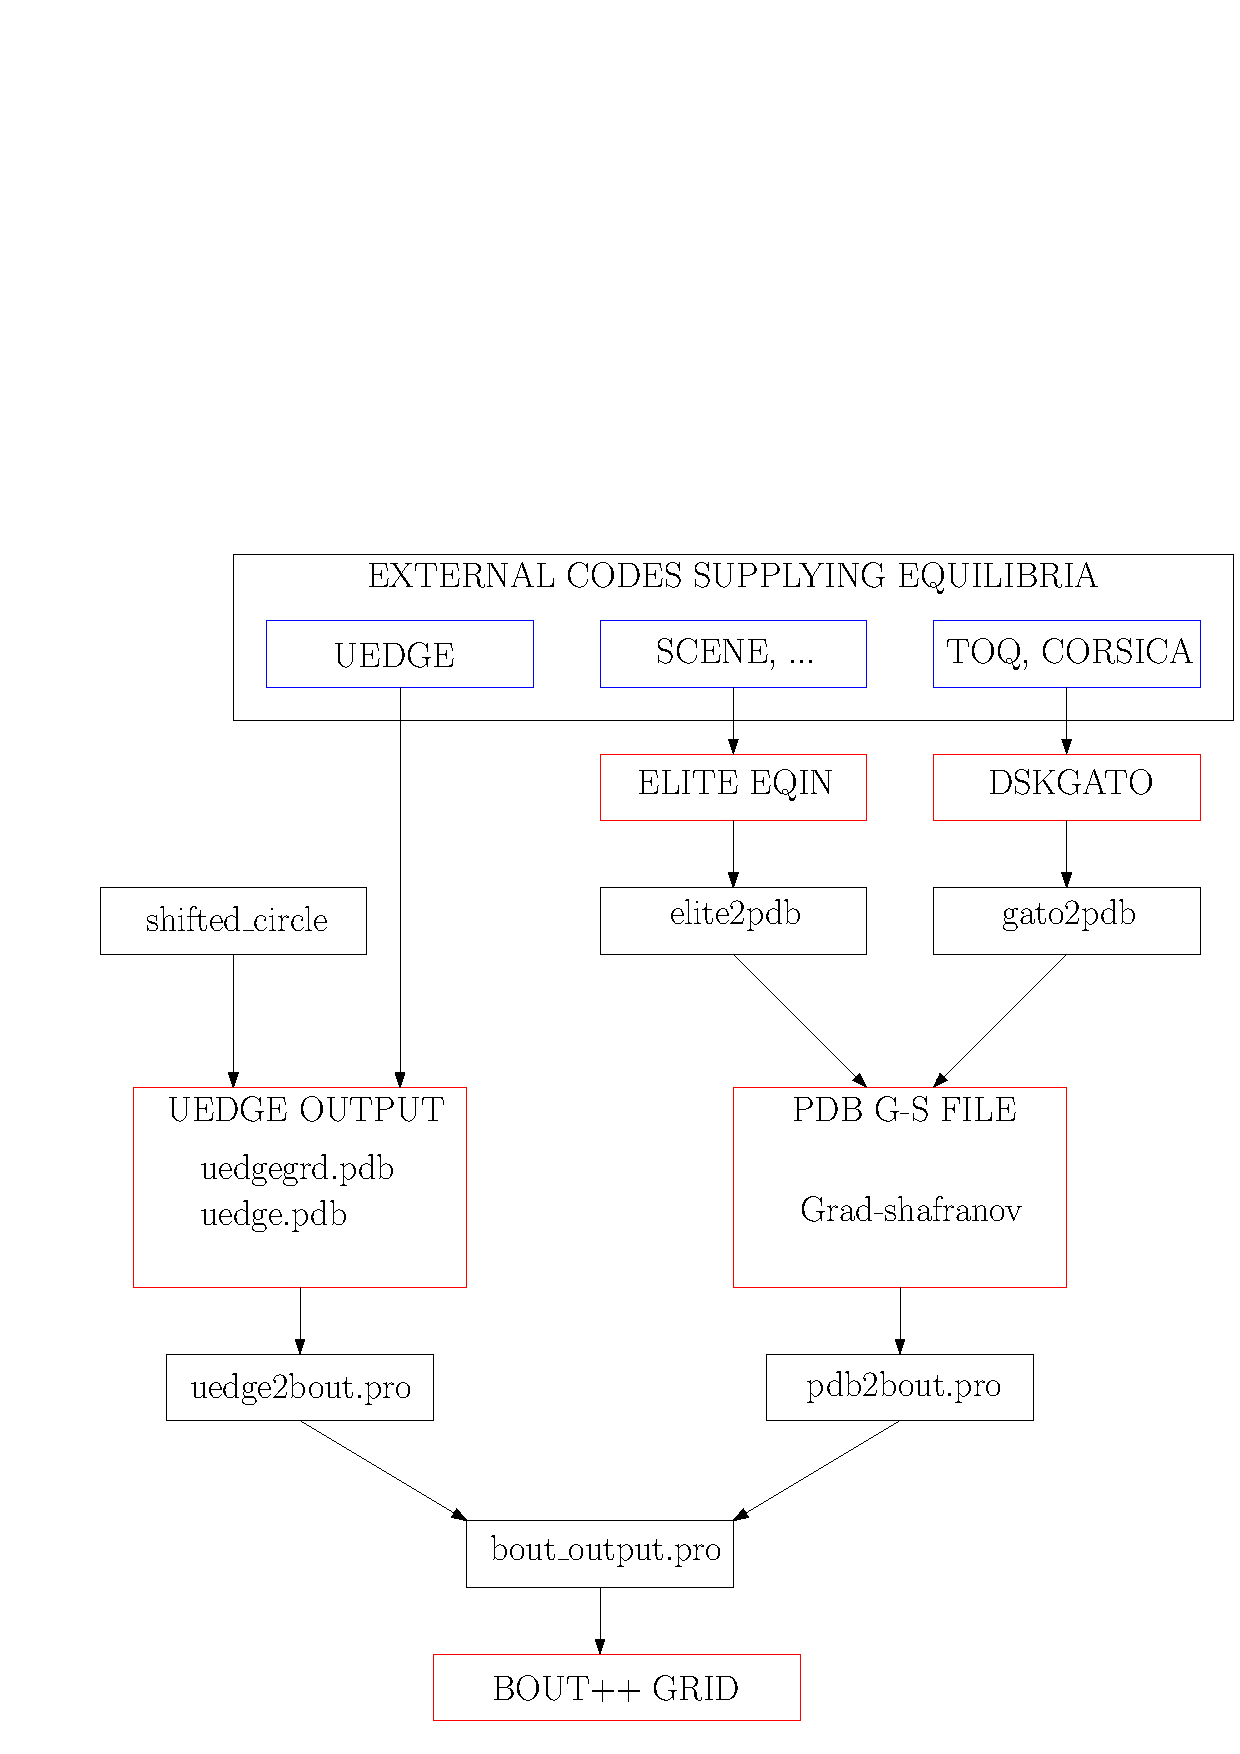
\includegraphics[width=0.7\paperwidth, keepaspectratio]{figs/grid_gen.pdf}
\caption{Generation of BOUT++ grid files. In red are the file formats, and in black the conversion routines. Blue are external codes.}
\label{fig:gridgen}
\end{figure}

\subsection{Converting grid files}

Currently conversions exist for ELITE \code{.eqin} and GATO \code{dskgato} equilibrium files.
Conversion of these into BOUT++ input grids is in two stages: In the first, both these
input files are converted into a common PDB format which describes the Grad-Shafranov equilibrium.
These intermediate files are then converted to BOUT++ grids using an interactive IDL script.


\subsection{Generating equilibria}

The directory \file{tokamak\_grids/shifted\_circle} contains IDL code to generate shifted circle
(large aspect ratio) Grad-Shafranov equilibria.

\subsection{Running pdb2bout}

There are many options which are set interactively, so here's a run-through of the code (only showing most important outputs):

\begin{verbatim}
IDL> pdb2bout, "cbm18_dens6.dskgato.pdb", output="test.pdb"
***Maximum mu0p is       23071.7
Is this pressure (not mu0*pressure)?
\end{verbatim}
This is needed because although many grid formats claim to store $\mu_0 P$, they actually store $P$. Since the given maximum value is very large, it must be in Pascals, so answer yes (y).

The grid will then be displayed along with the safety factor and pressure
profiles against normalised $\psi$. In all three plots, a red line marks the
location of the plasma edge. You must then choose the radial domain in normalised $\psi$:
\begin{verbatim}
Inner Psi boundary:0.6
Outer Psi boundary:1.2
Number of radial grid points:           69
Of which inside the plasma:           49
Is this range ok?
\end{verbatim}
The plots will now also show two green lines for the inner and outer boundaries. Enter no (n) to specify a different range.

The code then checks to see if any plasma density of temperatures have been set in the input file:
\begin{verbatim}
====== SETTING PLASMA PROFILES =======
Some plasma parameters given in input file
Use given parameters?
\end{verbatim}
Saying yes will just use the given values, but saying no will give you some more options:
\begin{verbatim}
Generating plasma profiles:
  1. Flat temperature profile
  2. Flat density profile
  3. Te proportional to density
Profile option:
\end{verbatim}
The procedure is the same for each of these, so taking option 2 (flat density):
\begin{verbatim}
Setting flat density profile
Density [10^20 m^-3]:1.0
\end{verbatim}
Anything can be entered here, depending on what you want to simulate. The code will ensure that whatever you enter, the equilibrium pressure is maintained. In this case the temperature is calculated from pressure and the specified density.
\begin{verbatim}
Maximum temperature (eV):      720.090
Is this ok?
\end{verbatim}
NOTE: This is the maximum temperature anywhere on the input grid (i.e. in this case at $\psi = 0$), not just inside the chosen domain. Entering no will go back and you can specify a different density.

Earlier the radial resolution was printed, in this case 69 grid points. You can now change this if you need to:
\begin{verbatim}
Increase radial resolution?
\end{verbatim}
Although it says increase, you can also decrease the resolution. Entering yes will allow you to enter a different number of radial grid points. It's recommended to use $2^n + 4$ grid points because this makes it easier to decompose the grid (4 cells for boundary, remainder equally divided between processors).

At this point, an orthogonal grid is generated:
\begin{verbatim}
======== GENERATING ORTHOGONAL COORDINATES FOR BOUT ========= 
Number of poloidal grid points: 64
Enter x index of equal hthe [0, 68] :35
\end{verbatim}
Using  $2^n$ points is highly recommended, but only because the points must be equally divided between processors.
The x index of equal hthe shouldn't matter very much except for highly shaped plasmas. Recommend that you set it somewhere around the peak pressure gradient, or middle of the grid.
\begin{verbatim}
Interpolating Rxy
Interpolating Zxy
Is this ok?
\end{verbatim}
Two plots are shown: On the left the original mesh, and on the right the new orthogonal mesh. If this doesn't look right you can enter `no' and change the poloidal resolution and location of equal $h_\theta$.

\begin{verbatim}
Add vacuum region?n
\end{verbatim}
This is a little experimental, and extends the grid into vacuum. This is useful if the equilibrium supplied doesn't include a vacuum region. In this case we already have a vacuum region, so can answer no.

You're now presented with several options:
\begin{verbatim}
Equilibrium correction options:
  0  No correction
  1  RBt using force balance
  2  hthe and RBt using force balance and q (FAILS)
  3  hthe and RBt using force balance and jpar
Enter option:
\end{verbatim}
Because the input Grad-shafranov solution is probably not perfect to begin with, and has now been interpolated onto a new grid, the force balance in ballooning coordinates is not quite satisfied. These options attempt to correct the equilibrium slightly to ensure force balance, the given $q$ profile, and the given $j_{||}$ profile. Option 1 can sometimes work well, other times it can fail to converge (as in this case). It's safe to just use option 0.

\begin{verbatim}
Calculating poloidal arc length dthe
Maximum difference in hthe:       0.23551123
Maximum percentage difference:        16.745859
Use new hthe?
\end{verbatim}
A key metric in the BOUT/BOUT++ coordinates is the poloidal arc length $h_\theta$. A plot will shot this quantity calculated geometrically (solid line), and calculated by enforcing force balance (red symbols) at the outboard midplane.
The difference between these two methods is an indication of the quality of the Grad-shafranov solution. Entering 'y' will use the ``new'' $h_\theta$ calculated from force balance, whilst 'n' will use the $h_\theta$ calculated geometrically. Personally. i prefer to make sure force balance is satisfied so enter 'y'.

\begin{verbatim}
Checking parallel current
****Equilibrium has -ve toroidal field
\end{verbatim}
Because of the varied and confusing ways different codes define the poloidal
and toroidal directions, this code currently just sets Bp and Bt positive,
and then uses the expression for Jpar to work out what sign Bt should have.
This is fine if you just want an equilibrium, but for detailed comparison to
experiment where the sign of Bt may/will make a difference this needs to be
changed.

Jpar calculated from quantities such as Bp, Bt and hthe is now shown as red symbols, with the jpar from the original Grad-shafranov solution as a black line. Like the hthe display, this is a good consistency check.
\begin{verbatim}
Use new Jpar?
\end{verbatim}
Entering 'y' will use the calculated jpar i.e. consistent with the other grid quantities, but probably more noisy and slightly different to the original. Entering 'n' will use the original jpar profiles.

\begin{verbatim}
q is negative. Reversing values from equilibrium
\end{verbatim}
This can be printed because the $q$ profile given in the grid file is almost always positive, whereas qsafe calculated by integrating the pitch angle can be positive or negative. In this case the toroidal field has been set negative (see above), and so qinty is negative too.

\begin{verbatim}
Use new qsafe?
\end{verbatim}
As with hthe and jpar, the qsafe specified in the original grid file is plotted as a black line, and the value calculated by integrating quantities on the new mesh is shown as red symbols. Entering 'y' uses the values consistent on the new grid, whilst 'n' uses the original safety factor profile. In most cases i'd prefer the grid to be consistent, rather than being identical to the input, so answer 'y'. You may have to do some experimentation though.

\begin{verbatim}
****Minimum pressure is very small:       0.0000000
****Setting minimum pressure to 1% of maximum
\end{verbatim}
This is because having negative pressures is very bad for BOUT/BOUT++ runs, and can easily be caused by overshoots or even rounding error when the pressure is too low. Because the equilibrium doesn't depend on absolute pressure, this just adds a constant pressure across the entire profile.

Finally, the grid file is written to PDB format
\begin{verbatim}
Cannot write 2 dimensional double dx. Writing as float
.
.
.
\end{verbatim}
These warnings are because the PDB2IDL library currently doesn't have any functions for writing doubles, and pdb2bout does calculations in double precision. The output is therefore converted to single-precision floats.

\section{Fluid equations}
\label{sec:equations}

Once you have tried some example codes, and generally got the hang of running
BOUT++ and analysing the results, there will probably come a time when
you want to change the equations being solved. 
This section uses the ideal MHD equations as an example, demonstrating how
a BOUT++ physics module is put together. It assumes you have a working knowledge
of C or C++, but you don't need to be an expert - most of the messy code is hidden away
from the physics module. There are several good books on C and C++, but I'd recommend online
tutorials over books because there are a lot more of them, they're quicker to scan through,
and they're cheaper.

When going through this section, it may help to refer to the finished code, which
is given in the file \file{mhd.cpp} in the BOUT++ examples directory. The equations to be solved are:
\begin{eqnarray*}
\deriv{\rho}{t} &=& -\mathbf{v}\cdot\nabla\rho - \rho\nabla\cdot\mathbf{v} \\
\deriv{p}{t} &=& -\mathbf{v}\cdot\nabla p - \gamma p\nabla\cdot\mathbf{v} \\
\deriv{\mathbf{v}}{t} &=& -\mathbf{v}\cdot\nabla\mathbf{v} + \frac{1}{\rho}\left(-\nabla p + \left(\nabla\times\mathbf{B}\right)\times\mathbf{B}\right) \\
\deriv{\mathbf{B}}{t} &=& \nabla\times\left(\mathbf{v}\times\mathbf{B}\right)
\end{eqnarray*}

To specify a set of equations to solve in BOUT++, two functions need to be written:
\begin{lstlisting}
int physics_init(bool restarting)
{
  return 0;
}

int physics_run(real t)
{
  return 0;
}
\end{lstlisting}
The first of these is called once at the start of the simulation, and should set up the problem,
specifying which variables are to be evolved. The argument \code{restarting} is false the first time a problem is run, and true if loading the state from a
restart file.

The second function \code{physics\_run} is called every time-step,
and should calculate the time-derivatives for a given state. In both cases returning non-zero
tells BOUT++ that an error occurred.

\subsection{Variables}

We need to define the variables to evolve as global variables (so they can be used in
\code{physics\_init} and \code{physics\_run}.

\note{Version 0.85 and earlier needed two variables to be defined, so if you're
upgrading then you can remove the time-derivative variables}

For ideal MHD, we need two 3D scalar fields density $\rho$ and pressure $p$, and two
3D vector fields velocity $v$, and magnetic field $B$:
\begin{lstlisting}
Field3D rho, p; // 3D scalar fields
Vector3D v, B;  // 3D vector fields

int physics_init(bool restarting)
{
}
\end{lstlisting}
For clarity, variables storing time-derivatives are here prefixed with \code{F\_}, but this is not
necessary - these variables can be named anything (as long as the name doesn't conflict with existing
global variables).

Scalar and vector fields behave much as you would expect: Field3D objects can be added, subtracted,
multiplied, divided and exponentiated, so the following examples are all valid operations:
\begin{lstlisting}
Field3D a, b, c;
real r;

a = b + c; a = b - c;
a = b * c; a = r * b;
a = b / c; a = b / r; a = r / b;
a = b ^ c; a = b ^ r; a = r ^ b;
\end{lstlisting}
Similarly, vector objects can be added/subtracted from each other, multiplied/divided by scalar
fields and real numbers, for example:
\begin{lstlisting}
Vector3D a, b, c;
Field3D f;
real r;

a = b + c; a = b - c;
a = b * f; a = b * r;
a = b / f; a = b / r;
\end{lstlisting}
In addition the dot and cross products are represented by \code{*} and \pow symbols:
\begin{lstlisting}
Vector3D a, b, c;
Field3D f;

f = a * b // Dot-product
a = b ^ c // Cross-product
\end{lstlisting}

For both scalar and vector field operations, so long as the result of an operation is of the correct type,
the usual C/C++ shorthand notation can be used:
\begin{lstlisting}
Field3D a, b;
Vector3D v, w;

a += b; v *= a; v -= w; v ^= w; // valid
v *= w; // NOT valid: result of dot-product is a scalar
\end{lstlisting}

%\parbox{\textwidth}

\note{In C++ the \pow operator has lower precedence than the \code{*} or \code{+} operators.
To be safe, always put exponentiation and cross-product operations in brackets}



\subsection{Evolution equations}

At this point we can tell BOUT++ which variables to evolve, and where the state and time-derivatives
will be stored. This is done using the \code{bout\_solve(variable, name)} function
in \code{physics\_init}:
\begin{lstlisting}
int physics_init(bool restarting)
{
  bout_solve(rho, "density");
  bout_solve(p,   "pressure");
  bout_solve(v,   "v");
  bout_solve(B,   "B");
  
  return 0;
}
\end{lstlisting}
The name given to this function will be used in the output and restart data files. These will be
automatically read and written depending on input options (see section~\ref{subsec:options}).
Input options based on these names are also used to initialise the variables.

The equations to be solved can now be written in the \code{physics\_run} function. The value
passed to the function (\code{real t}) is the simulation time - only needed if your
equations contain time-dependent sources or similar terms. To refer to the time-derivative
of a variable \code{var}, use \code{ddt(var)}. The ideal MHD equations can be written as:
\begin{lstlisting}
int physics_run(real t)
{
  ddt(rho) = -V_dot_Grad(v, rho) - rho*Div(v);
  ddt(p) = -V_dot_Grad(v, p) - gamma*p*Div(v);
  ddt(v) = -V_dot_Grad(v, v) + ( (Curl(B)^B) - Grad(p) ) / rho;
  ddt(B) = Curl(v^B);
}
\end{lstlisting}
Where the differential operators \code{vector = Grad(scalar)}, \code{scalar = Div(vector)}, and
\code{vector = Curl(vector)} are used. For the density and pressure equations, 
the $\mathbf{v}\cdot\nabla\rho$ term could be written as \code{v*Grad(rho)}, but this would then use
central differencing in the Grad operator. Instead, the function \code{V\_dot\_Grad} uses upwinding
methods specifically for these advection terms. In addition, the \code{Grad} function will not operate
on vector objects (since result is neither scalar nor vector), so the $\mathbf{v}\cdot\nabla\mathbf{v}$ term CANNOT be written as \code{v*Grad(v)}. 

\subsection{Input options}
\label{sec:inputopts}

Note that in the above equations the extra parameter \code{gamma} has been used. To enable this to be set
in the input options file (see section~\ref{sec:options}), we use the \code{options} object in the
initialisation function:
\begin{lstlisting}
real gamma;

int physics_init(bool restarting)
{
  options.get("mhd", "gamma", gamma, 5.0/3.0);
\end{lstlisting}
This specifies that an option called ``gamma'' in a section called ``mhd'' should be put into the variable \code{gamma}. If the option could not be found, or was of the wrong type, the variable should be set to a default value of $5/3$.
The value used will be printed to the output file, so if gamma is not set in the input file the following line will appear:
\begin{verbatim}
      Option mhd / gamm = 1.66667 (default)
\end{verbatim}
This function can be used to get integers and booleans. To get strings, there
is the function (\code{char* options.getString(section, name)}.
To separate options specific to the physics model, these options should be put in a separate
section, for example here the ``mhd'' section has been specified. To save having to write the section name for every option, there is the \code{setSection} function:
\begin{lstlisting}
real gamma;
int someint;

int physics_init(bool restarting)
{
  options.setSection("mhd");
  options.get("gamma",   gamma,   5.0/3.0);
  options.get("someint", someint, 0);
\end{lstlisting}
Most of the time, the name of the variable (e.g. \code{gamma}) will be
the same as the identifier in the options file (``gamma''). In this case,
there is the macro
\begin{lstlisting}
OPTION(gamma, 5.0/3.0);
\end{lstlisting}
which is equivalent to
\begin{lstlisting}
options.get("gamma",   gamma,   5.0/3.0);
\end{lstlisting}
See section~\ref{sec:options} for more details of how to use the input options.

\subsection{Communication}

If you plan to run BOUT++ on more than one processor, any operations involving y derivatives
will require knowledge of data stored on other processors. To handle the necessary parallel
communication, there is the \code{mesh->communicate} function. This takes care of where the data
needs to go to/from, and only needs to be told which variables to transfer.

If you only need to communicate a small number (up to 5 currently) of variables then just
call the \code{mesh->communicate} function directly. For the MHD code, we need to communicate
the variables \code{rho,p,v,B} at the beginning of the \code{physics\_run} function
before any derivatives are calculated:
\begin{lstlisting}
int physics_run(real t)
{
  mesh->communicate(rho, p, v, B);
\end{lstlisting}

If you need to communicate lots of variables, or want to change at run-time which
variables are evolved (e.g. depending on input options), then you can create a group
of variables and communicate them later.
To do this, first create a \code{FieldGroup} object, in this case called \code{comms},
then use the add method. This method does no communication, but records which variables to transfer
when the communication is done later.
\begin{lstlisting}
FieldGroup comms;

int physics_init()
{
  .
  .
  .
  comms.add(rho);
  comms.add(p);
  comms.add(v);
  comms.add(B);

  return 0;
}
\end{lstlisting}

To perform the actual communication, call the \code{mesh->communicate} function
with the group. In this case
we need to communicate all these variables before performing any calculations, so call
this function at the start of the \code{physics\_run} routine:
\begin{lstlisting}
int physics_run(real t)
{
  mesh->communicate(comms);
  .
  .
  .
\end{lstlisting}
In many situations there may be several groups of variables which can be communicated at
different times. The function \code{mesh->communicate} consists of a call to \code{mesh->send} followed by \code{mesh->wait}
which can be done separately to interleave calculations and communications. This will speed up the
code if parallel communication bandwidth is a problem for your simulation.

In our MHD example, the calculation of \code{ddt(rho)} and \code{ddt(p)} does not require
\code{B}, so we could first communicate \code{rho}, \code{p}, and \code{v}, send \code{B}
and do some calculations whilst communications are performed:
\begin{lstlisting}
int physics_run(real t)
{
  mesh->communicate(rho, p, v); // sends and receives rho, p and v
  comm_handle ch = mesh->send(B);// only send B
  
  ddt(rho) = ...
  ddt(p) = ...
  
  mesh->wait(ch); // now wait for B to arrive
  
  ddt(v) = ...
  ddt(B) = ...

  return 0;
}
\end{lstlisting}

This scheme is not used in \file{mhd.cpp}, partly for clarity, and partly because currently
communications are not a significant bottleneck (too much inefficiency elsewhere!).

\note{1. Before using the result of a differential operator as input to another differential operator,
communications must be performed for the intermediate result \\
2. Currently communicator objects cannot overlap: Only one communicator object can be in the middle of a
send-receive pair at any given time. Calling \code{comms1.send(); comms2.send();} will cause
chaos. This is a bug which will be fixed in future.}

\subsection{Initial profiles}

Up to this point the code is evolving total density, pressure etc. This has advantages for clarity,
but has problems numerically: For small perturbations, rounding error and tolerances in the time-integration
mean that linear dispersion relations are not calculated correctly. The solution to this
is to write all equations in terms of an initial ``background'' quantity and a time-evolving
perturbation, for example $\rho\left(t\right) \rightarrow \rho_0 + \tilde{\rho}\left(t\right)$.
For this reason, {\bf the initialisation of all variables passed to the \code{bout\_solve} function
is a combination of small-amplitude gaussians and waves; the user is expected to have performed this
separation into background and perturbed quantities.} 

To read in a quantity from a grid file, there is the \code{grid.get} function:

\begin{lstlisting}
Field2D Ni0; // Background density

int physics_init(bool restarting)
{
  ...
  mesh->get(Ni0, "Ni0");
  ...
}
\end{lstlisting}

As with the input options, most of the time the name of the variable in the
physics code will be the same as the name in the grid file to avoid confusion.
In this case, you can just use
\begin{lstlisting}
GRID_LOAD(Ni0);
\end{lstlisting}
which is equivalent to
\begin{lstlisting}
mesh->get(Ni0, "Ni0");
\end{lstlisting}

\subsection{Boundary conditions}

In addition to the equations to be solved, we need to specify the boundary conditions
for each of the variables. The simplest way to do this is to use the \code{apply\_boundary}
function, and then set the condition to be used in the input file.


\subsection{Other components}

The MHD example presented previously covered many of the functions available in BOUT++,
which can be used for a wide variety of models. There are however several other significant
functions and classes which deserve a mention here. For a full listing, see the reference manual.

\subsubsection{Printing messages/warnings}
\label{sec:printing}

In order to print to screen and/or a log file, the object \code{output} is provided. 
This provides two different ways to write output: the C (\code{printf}) way, and the
C++ stream way. This is because each method can be clearer in different circumstances,
and people have different tastes in these matters. 

The C-like way (which is the dominant way in BOUT++) is to use the \code{write} function,
which works just like \code{printf}, and takes all the same codes (it uses \code{sprintf}
internally). 
\begin{lstlisting}
output.write(const char *format, ...)
\end{lstlisting}
For example:
\begin{lstlisting}
output.write("This is an integer: %d, and this a real: %e\n", 5, 2.0)
\end{lstlisting}

For those who prefer the C++ way of doing things, a completely equivalent way is to
treat \code{output} as you would \code{cout}:
\begin{lstlisting}
output << "This is an integer: " << 5 << ", and this a real: " << 2.0 << endl;
\end{lstlisting}
which will produce exactly the same result as the \code{output.write} call above.

On all processors, anything sent to \code{output} will be written to a log file called
\file{BOUT.log.\#} with \# replaced by the processor number. On processor 0, anything
written to the output will be written to screen (stdout), in addition to the log file.
Unless there is a really good reason not to, please use this \code{output} object 
when writing text output.

\subsubsection{Laplacian inversion}

Quite a common problem in plasma simulation codes is to invert an equation of the form
\[
\nabla_\perp^2 x + a x = b
\]
where $a$ is symmetric in z, and the operator $\nabla_\perp = \nabla - \mathbf{b}\left(\mathbf{b}\cdot\nabla\right) = -\mathbf{b\times} \left(\mathbf{b\times}\nabla\right)$. For example, this operator
appears in reduced MHD for the vorticity inversion and $j_||$.
Efficiently inverting this operator is done in the same way as in the BOUT code:
FFTs are used in the $z$ direction to transform this problem into a set of 1D 
inversion problems (in $x$) for each Fourier mode.
These inversion problems are band-diagonal (tri-diagonal in the case of 2nd-order differencing) and so
inversions are very efficient: $O\left(n_z \log n_z\right)$ for the FFTs, $O\left(n_x\right)$ for tridiagonal inversion
using the Thomas algorithm \cite{press-1999}, where $n_x$ and $n_z$ are the number of grid-points
in the $x$ and $z$ directions respectively.
This routine is:
\begin{lstlisting}
invert_laplace(b, x, flags, &a);
\end{lstlisting}
where \code{b} and \code{x} are 3D fields, and \code{a} is a pointer to a 2D field (which may be
NULL). \code{flags} is an \code{int} which determines boundary conditions and other options.
Its value is calculated by adding the settings given in \code{invert\_laplace.h}, and reproduced in
table~\ref{tab:laplaceflags}.
\begin{table}[htbp!]
\caption{Laplacian inversion flags: add the required quantities together.}
\label{tab:laplaceflags}
\centering
\begin{tabular}[c]{c | l}
\hline
Flag & Meaning \\
\hline
1 & Zero-gradient DC on inner (X) boundary. Default is zero-value \\
2 & Zero-gradient AC on inner boundary \\
4 & Zero-gradient DC on outer boundary \\
8 & Zero-gradietn AC on outer boundary \\
16 & Zero DC component everywhere \\
32 & Not used currently \\
64 & Set width of boundary to 1 (default is \code{MXG}) \\
128 & Use 4$^{th}$-order band solver (default is 2$^{nd}$ order tridiagonal) \\
256 & Attempt to set zero laplacian AC component on inner boundary by combining \\
    & 2nd and 4th-order differencing at the boundary. \\
    & Ignored if tridiagonal solver used. \\
512 & Zero laplacian AC on outer boundary \\
1024 & Symmetric boundary condition on inner boundary \\
2048 & Symmetric outer boundary condition \\
\hline
\end{tabular}
\end{table}

\subsubsection{Error handling}

Finding where bugs have occurred in a (fairly large) parallel code is a difficult problem.
This is more of a concern for developers of BOUT++ (see the developers manual), but it is still
useful for the user to be able to hunt down bug in their own code, or help narrow down where
a bug could be occurring.

If you have a bug which is easily reproduceable i.e. it occurs almost immediately every time
you run the code, then the easiest way to hunt down the bug is to insert lots of \code{output.write}
statements (see section~\ref{sec:printing}). Things get harder when a bug only occurs after a long time
of running, and/or only occasionally. For this type of problem, a useful tool
can be the message stack.
At the start of a section of code, put a message onto the stack:
\begin{lstlisting}
   msg_stack.push("Some message here");
\end{lstlisting}
which can also take arguments in \code{printf} format, as with \code{output.write}. At the end of the section of code, take the message off the stack again:
\begin{lstlisting}
   msg_stack.pop();
\end{lstlisting}
If an error occurs, the message stack is printed out, and this can then
help track down where the error originated.


\section{Differential operators}
\label{sec:diffops}

There are a huge number of possible ways to perform differencing in computational
fluid dynamics, and BOUT++ is intended to be able to implement a large number of them. This
means that the way differentials are handled internally is quite involved; see the
developer's manual for full gory details. Much of the time this detail is not all that
important, and certainly not while learning to use BOUT++. Default options are
therefore set which work most of the time, so you can start using the code without
getting bogged down in these details.

In order to handle many different differencing methods and operations, many layers are
used, each of which handles just part of the problem. The main division is between
differencing methods (such as 4th-order central differencing), and differential operators
(such as $\nabla_{||}$).

\subsection{Differencing methods}

Methods used can be divided into central-differencing and upwinding methods. Central
methods currently implemented are:
\begin{itemize}
\item 2nd-order
\item 4th-order
\item FFT for Z (symmetry) direction.
\end{itemize}
These are used for diffusion-type operators, and almost always the higher-accuracy 4th-order
and FFT methods are used.

Upwinding methods available for advection-type operators are
\begin{itemize}
\item 1st-order upwinding
\item 3rd-order Weighted Essentially Non-Oscillatory (WENO)\cite{jiang-1997}
\end{itemize}
Both of these methods avoid overshoots (Gibbs phenomena) at sharp gradients such as shocks,
but the simple 1st-order method has very large artificial diffusion. WENO schemes are
a development of the ENO reconstruction schemes which combine good handling of sharp-gradient
regions with high accuracy in smooth regions.

\subsection{Operators}

These are differential operators which are independent of the coordinate system used.
\[
\begin{array}{rclrcl}
\mathbf{v} &=& \nabla f &\qquad \code{Vector} &=& \code{Grad(Field)} \\
f &=& \nabla\cdot\mathbf{a} &\qquad \code{Field} &=& \code{Div(Vector)} \\
\mathbf{v} &=& \nabla\times\mathbf{a} &\qquad \code{Vector} &=& \code{Curl(Vector)} \\
f &=& \mathbf{v}\cdot\nabla g &\qquad \code{Field} &=& \code{V\_dot\_Grad(Vector, Field)} \\
\mathbf{v} &=& \mathbf{a}\cdot\nabla\mathbf{b} &\qquad \code{Vector} &=& \code{V\_dot\_Grad(Vector, Vector)} \\
f &=& \nabla^2 f &\qquad \code{Field} &=& \code{Laplacian(Field)}
\end{array}
\]

\begin{eqnarray*}
\nabla\phi &=& \deriv{\phi}{u^i}\nabla u^i \Rightarrow \left(\nabla\phi\right)_i = \deriv{\phi}{u^i} \\
\nabla\cdot A &=& = \frac{1}{J}\deriv{}{u^i}\left(Jg^{ij}A_j\right) \\
\nabla^2\phi &=& \Gamma^i\deriv{\phi}{u^i} + g^{ij}\frac{\partial^2\phi}{\partial u^i\partial u^j} \\
& &\Gamma^i = \frac{1}{J}\deriv{}{u^i}\left(Jg^{ij}\right)
\end{eqnarray*}

Another set of operators assume that the equilibrium magnetic field is written
in Clebsh form as
\[
\mathbf{B}_0 = \nabla z\times\nabla x \qquad \left|B_0\right| = \frac{\sqrt{g_{yy}}}{J}
\]

\begin{eqnarray*}
\partial^0_{||} &=& \mathbf{b}_0\cdot\nabla = \frac{1}{\sqrt{g_{yy}}}\deriv{}{y} \\
\nabla^0_{||}F &=& B_0\partial^0_{||}\left(\frac{F}{B_0}\right) \\
\partial^2_{||}\phi &=& \partial^0_{||}\left(\partial^0_{||}\phi\right) = \frac{1}{\sqrt{g_{yy}}}\deriv{}{y}\left(\frac{1}{\sqrt{g_{yy}}}\right)\deriv{\phi}{y} + \frac{1}{g_{yy}}\frac{\partial^2\phi}{\partial y^2} \\
\mathbf{b}_0\cdot\nabla\phi\times\nabla A &=& \frac{1}{J\sqrt{g_{yy}}}\left[\left(g_{yy}\deriv{\phi}{z} - g_{yz}\deriv{\phi}{y}\right)\deriv{A}{x} + \left(g_{yz}\deriv{\phi}{x} - g_{xy}\deriv{\phi}{z}\right)\deriv{A}{y} + \left(g_{xy}\deriv{\phi}{y} - g_{yy}\deriv{\phi}{x}\right)\deriv{A}{z}\right]
\end{eqnarray*}

\subsection{Setting differencing method}

\section{Staggered grids}
\label{sec:staggergrids}

Until now all quantities have been cell-centred i.e. both velocities
and conserved quantities were defined at the same locations. This
is because these methods are simple and this was the scheme used in 
the original BOUT. This class of methods can however be susceptable to
grid-grid oscillations, and so most shock-capturing schemes involve
densities and velocities (for example) which are not defined at the same location: their
grids are staggered.

By default BOUT++ runs with all quantities at cell centre. To enable staggered grids,
set
\begin{verbatim}
StaggeredGrids = true
\end{verbatim}
in the top section of the \file{BOUT.inp} file.

There are four possible locations in a grid cell where a quantitity can be defined in BOUT++:
centre, lower X, lower Y, and lower Z. These are illustrated in figure~\ref{fig:stagLocations}.
\begin{figure}[htbp!]
\centering
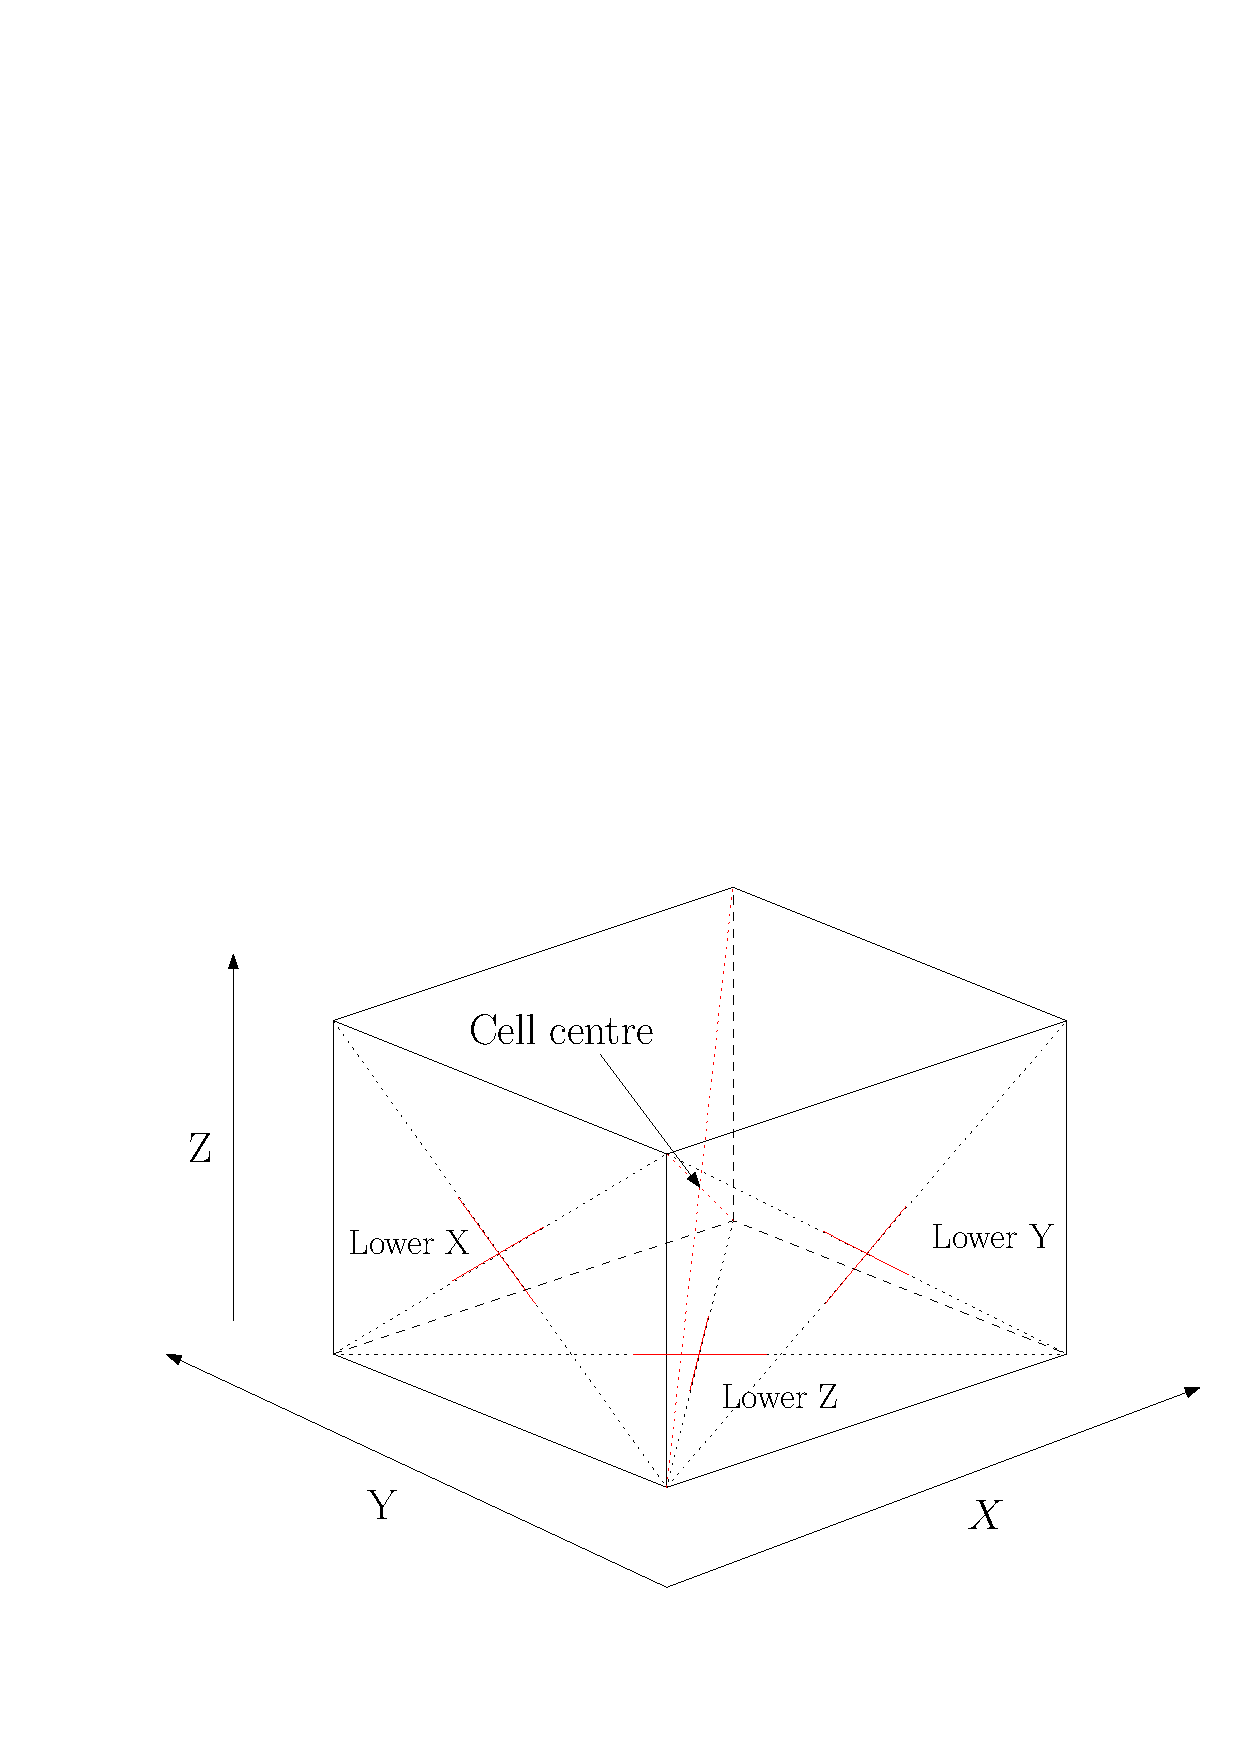
\includegraphics[width=0.4\paperwidth, keepaspectratio]{figs/stagLocations.pdf}
\caption{Locations in a grid cell where quantities may be defined.}
\label{fig:stagLocations}
\end{figure}

\begin{figure}[htbp!]
\centering
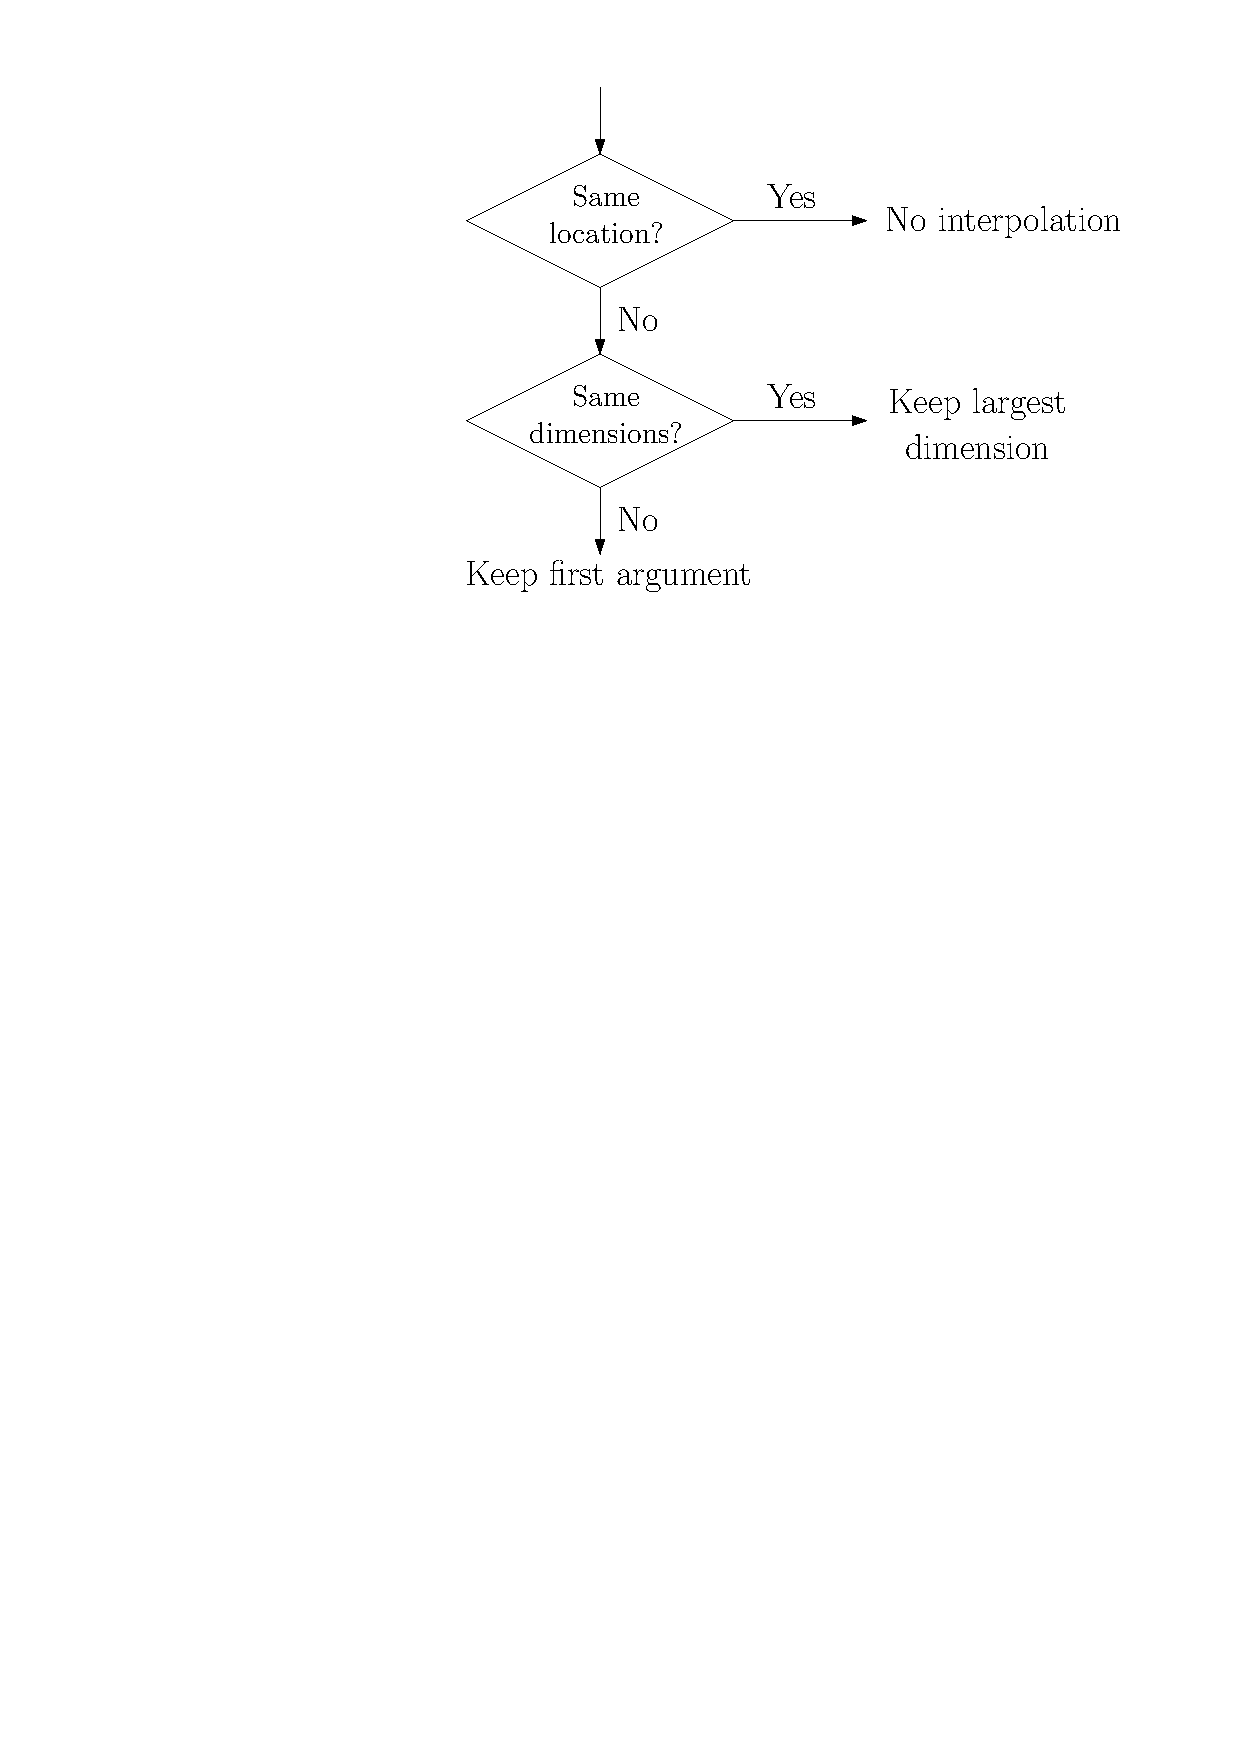
\includegraphics[width=0.4\paperwidth, keepaspectratio]{figs/stagArith.pdf}
\caption{How the cell location of an arithmetic operation (\code{+,-,*,/,\pow}) is decided}
\label{fig:stagArith}
\end{figure}




\section{Examples}
\label{sec:examples}

\subsection{Linear device}

This test-case is a simplified simulation of turbulence in a linear plasma device. 

\subsection{2-Fluid Braginskii}

The physics code \file{2fluid.cpp} implements a set of reduced Braginskii 2-fluid equations,
similar to those solved by the original BOUT code.
This evolves 6 variables: Density, electron and ion temperatures, parallel ion velocity,
parallel current density and vorticity.

Input grid files are the same as the original BOUT code, but the output format is different.

\subsection{Reduced MHD}

The file \file{highbeta\_reduced.cpp} solves for a reduced single-fluid MHD similar to that
derived in \cite{hazeltine-2003} (flute-reduced, page 282), used for linear ELM modelling.
A separate document \file{elm\_reduced.pdf} in this manual directory derives and explains
the model and coordinate system used.

\subsection{Compressible Fluid}

The model in \file{gas\_compress.cpp} solves the compressible gas dynamics equations for
the density $n$, velocity $\mathbf{V}$, and pressure $P$:

\subsection{MHD}

The file \file{mhd.cpp} solves the full MHD equations for the full values (perturbation + initial),
whilst the file \file{mhd\_perturb.cpp} solves for a perturbation about the equilibrium.

\section{Notes}

\subsection{Compile options}

Compiling with \code{-DCHECK} enables a lot of checks of operations performed by the field
objects. This is very useful for debugging a code, and can be omitted once bugs have been removed.

For (sometimes) more useful error messages, there is the \code{-DTRACK} option. This
keeps track of the names of variables and includes these in error messages.

\subsection{Adaptive grids}

Two types of adaptive grids can be used in BOUT++: Moving meshes, and changing resolution.

\subsubsection{Moving meshes}

During either the initialisation, or the simulation itself, the metric tensors can be modified. This could
be used to make the coordinate system time-dependent. Since currently the metric tensors are 2D
fields, this would only allow axi-symmetric motion. Changing the tensors to be 3D objects is however
possible with fairly small modification to the code.

Whenever one of the metrics $g^{ij}$ are changed, a call to \code{geometry()} must be made.

\subsubsection{Changing resolution}

\note{Not implemented yet - this just for discussion}

Since all 2D and 3D fields/vectors are located internally in global lists, the resolution
of the grid can be changed when required by interpolation. {\bf This requires a new, more
efficient implementation of the Fields classes}.

\bibliography{references}
\bibliographystyle{unsrt}

\appendix

\section{Installing PACT}
\label{apx:pact}

There are two ways to install PACT, and usually one of them will 
work on a given system. 

\subsection{Self-extracting package}

This is probably the easiest method (when it works). Download one of the 
``Executable UNIX distribution files'' from the PACT website and run:
\begin{verbatim}
./pact07_07_18-src -sl -i $HOME/local/
\end{verbatim}
The ``-sl'' flag tells it to generate shared libraries. If you don't plan on using IDL
to read/write PDB files, then you can omit this. The ``-i \$HOME/local/'' tells PACT to install
in your home directory/local.

If this script fails, you will usually have to resort to either trying to understand
DSYS, or going with the second method below.

\subsection{PACT source distribution}

The second method is to use a .tar.gz PACT source file. Here the version used
is \file{pact-2.1.0.tar.gz}.

\begin{verbatim}
 ~/ $ cd install
 ~/install/ $ tar -xzvf pact-2.1.0.tar.gz
 ~/install/ $ cd pact-2.1.0/
 ~/install/pact-2.1.0/ $ ./configure --prefix=$HOME/local --enable-shared
\end{verbatim}

\note{On Franklin, PACT will compile without the --enable-shared option, but not with it. This is OK if you just want to run BOUT++, but the shared libraries are needed for reading the results into IDL (the PDB2IDL library)}

At this point, the installation may fail with the following error:
\begin{verbatim}
configure: WARNING: yacc is a symbolic link to bison
configure: WARNING: bison is not a supported type of yacc
configure: error: No working yacc found
\end{verbatim}

If this happens, you need to first install Berkeley Yacc into your home directory
\begin{verbatim}
 ~/install/ $ ls
byacc.tar.gz       netcdf-tar -xzvf byacc.tar.gz4.0.1.tar.gz  pact-2.1.0.tar.gz
fftw-3.2.1.tar.gz  pact-2.1.0           sundials-2.4.0.tar.gz

 ~/install/ $ tar -xzvf byacc.tar.gz
 ~/install/ $ cd byacc-20080826/
 ~/install/byacc-20080826/ $ ./configure --prefix=$HOME/local
 ~/install/byacc-20080826/ $ gmake
 ~/install/byacc-20080826/ $ mkdir ~/local/bin
 ~/install/byacc-20080826/ $ cp yacc ~/local/bin/
\end{verbatim}
NB: We're copying the yacc executable manually because ``gmake install'' doesn't seem to work,
and the fix which works for PACT (see later) doesn't work here.

Add this directory to your path:
\begin{verbatim}
 ~/install/byacc-20080826/ $ setenv PATH $HOME/local/bin:$PATH
\end{verbatim}
You can check that this has worked by running ``which yacc'', which should then print
your home directory /local/bin/yacc.
You could also add this to your .profile startup scripts. Now go back to PACT:
\begin{verbatim}
 ~/install/byacc-20080826/ $ cd ../pact-2.1.0
 ~/install/pact-2.1.0/ $ ./configure --prefix=$HOME/local --enable-shared
 ~/install/pact-2.1.0/ $ gmake
 ~/install/pact-2.1.0/ $ gmake install
\end{verbatim}

The last step may fail with a strange error message like:
\begin{verbatim}
    The current directory must be set to the ITT directory.
    Change the default to the ITT directory and re-run
    this script.
\end{verbatim}
This happens when the wrong ``install'' is being used. Check by running:
\begin{verbatim}
 ~/install/byacc-20080826/ $ which install
\end{verbatim}
This should print ``/usr/bin/install'', but if not then run
\begin{verbatim}
 ~/install/byacc-20080826/ $ ln -s /usr/bin/install ~/local/bin/
 ~/install/pact-2.1.0/ $ ./configure --prefix=$HOME/local
 ~/install/pact-2.1.0/ $ gmake
 ~/install/pact-2.1.0/ $ gmake install
\end{verbatim}
NOTE: configure needs to be run again after messing with install.

This should now install PACT into your local directory.

\section{Compiling and running under AIX}

Most development and running of BOUT++ is done under Linux, with the occasional FreeBSD and OSX.
The configuration scripts are therefore heavily tested on these architectures. IBM's POWER
architecture however runs AIX, which has some crucial differences which make compiling a pain.

\begin{itemize}
\item Under Linux/BSD, it's usual for a Fortran routine \code{foo} to appear
  under C as \code{foo\_}, whilst under AIX the name is unchanged
\item MPI compiler scripts are usually given the names \code{mpicc} and
  either \code{mpiCC} or \code{mpicxx}. AIX uses \code{mpcc} and \code{mpCC}.
\item Like BSD, the \code{make} command isn't compatible with GNU make,
  so you have to run \code{gmake} to compile everything.
\item The POWER architecture is big-endian, different to the little endian 
  Intel and AMD chips. This can cause problems with binary file formats.
\end{itemize}

\subsection{SUNDIALS}

To compile SUNDIALS, use 
\begin{verbatim}
$ export CC=cc
$ export CXX=xlC
$ export F77=xlf
$ export OBJECT_MODE=64
$ ./configure --prefix=$HOME/local/ --with-mpicc=mpcc --with-mpif77=mpxlf CFLAGS=-maix64
\end{verbatim}

You may get an error message like:
\begin{verbatim}
make: Not a recognized flag: w
\end{verbatim}
This is because the AIX \code{make} is being used, rather than \code{gmake}.
The easiest way to fix this is to make a link to \code{gmake} in your local
bin directory:
\begin{verbatim}
$ ln -s /usr/bin/gmake $HOME/local/bin/make
\end{verbatim}
Running \code{which make} should now point to this \code{local/bin/make},
and if not then you need to make sure that your bin directory appears first
in the \code{PATH}:
\begin{verbatim}
export PATH=$HOME/local/bin:$PATH
\end{verbatim}

If you see an error like this:
\begin{verbatim}
ar: 0707-126 ../../src/sundials/sundials_math.o is not valid with the current object file mode.
        Use the -X option to specify the desired object mode.
\end{verbatim}
then you need to set the environment variable \code{OBJECT\_MODE}
\begin{verbatim}
export OBJECT_MODE=64
\end{verbatim}

Configuring BOUT++, you may get the error:
\begin{verbatim}
configure: error: C compiler cannot create executables
\end{verbatim}
In that case, you can try using:
\begin{verbatim}
./configure CFLAGS="-maix64"
\end{verbatim}

When compiling, you may see warnings
\begin{verbatim}
xlC_r: 1501-216 (W) command option -64 is not recognized - passed to ld
\end{verbatim}

At this point, the main BOUT++ library should compile, and you can try
compiling one of the examples. 

\begin{verbatim}
ld: 0711-317 ERROR: Undefined symbol: .NcError::NcError(NcError::Behavior)
ld: 0711-317 ERROR: Undefined symbol: .NcFile::is_valid() const
ld: 0711-317 ERROR: Undefined symbol: .NcError::~NcError()
ld: 0711-317 ERROR: Undefined symbol: .NcFile::get_dim(const char*) const
\end{verbatim}

This is probably because the NetCDF libraries are 32-bit, whilst BOUT++ has been compiled as 64-bit. 
You can try compiling BOUT++ as 32-bit:
\begin{verbatim}
$ export OBJECT_MODE=32
$ ./configure CFLAGS="-maix32"
$ gmake
\end{verbatim}
If you still get undefined symbols, then go back to 64-bit, and edit make.config, raplacing
\code{-lnetcdf\_c++} with {-lnetcdf64\_c++}, and \code{-lnetcdf} with {-lnetcdf64}. This 
can be done by running:
\begin{verbatim}
$ sed 's/netcdf/netcdf64/g' make.config > make.config.new
$ mv make.config.new make.config
\end{verbatim}

\section{BOUT++ functions (alphabetical)}

This is a list of functions which can be called by users writing
a physics module. For a full list of functions, see the Reference manual,
DOxygen documentation, and source code.

\begin{itemize}
  \item \texttt{Field = {\bf abs}(Field | Vector)}
  \item \texttt{(Communicator).{\bf{add}}(Field | Vector)} \\
    Add a variable to a communicator object.
  \item \texttt{{\bf apply\_boundary}(Field. ``name'')}
  \item \texttt{Field = {\bf b0xGrad\_dot\_Grad}(Field, Field, CELL\_LOC)}
  \item \texttt{{\bf bout\_solve}(Field, Field, ``name'')}
  \item \texttt{{\bf bout\_solve}(Vector, Vector, ``name'')}
  \item \texttt{(Communicator).{\bf{clear}}()} \\
    Remove all variables from a Communicator object
  \item \texttt{Field = {\bf cos}(Field)}
  \item \texttt{Field = {\bf cosh}(Field)}
  \item \texttt{Vector = {\bf Curl}(Vector)}
  \item \texttt{Field = {\bf Delp2}(Field)} \\
    $\nabla_\perp^2$ operator
  \item \texttt{Field = {\bf Div}(Vector)} \\
    Divergence of a vector
  \item \texttt{Field = {\bf Div\_par}(Field f)} \\
    Parallel divergence $B_0\mathbf{b}\cdot\nabla\left(f / B_0\right)$
  \item \texttt{{\bf dump.add}(Field, ``name'', 1/0)}
  \item \texttt{Field = {\bf filter}(Field, modenr)}
  \item \texttt{{\bf geometry\_derivs}()} \\
    Calculates useful quantities from the metric tensor. Call this
    every time the metric tensor is changed.
  \item \texttt{Vector = {\bf Grad}(Field)}
  \item \texttt{Field = {\bf Grad\_par}(Field)}
  \item \texttt{Field = {\bf Grad2\_par2}(Field)}
  \item \texttt{{\bf grid\_load}(real, ``name'')} \\
    Load a scalar real from the grid file
  \item \texttt{{\bf grid\_load2d}(Field2D, ``name'')} \\
    Load a 2D scalar field from the grid file
  \item \texttt{{\bf grid\_load3d}(Field3D, ``name'')} \\
    Load a 3D scalar field from the grid file
  \item \texttt{{\bf invert\_laplace}(Field input, Field output, flags, Field2D *A)}
  \item \texttt{Field = {\bf invert\_parderiv}(Field2D|real A, Field2D|real B, Field3D r)} \\
    Inverts an equation  \code{A*x + B*Grad2\_par2(x) = r}
  \item \texttt{Field = {\bf Laplacian}(Field)}
  \item \texttt{Field3D = {\bf low\_pass}(Field3D, max\_modenr)}
  \item \texttt{real = {\bf max}(Field)}
  \item \texttt{real = {\bf min}(Field)}
  \item \texttt{{\bf msg\_stack.pop}( |int)} \\
    Remove a message from the top of the stack. If a message ID is passed,
    removes all messages back to that point.
  \item \texttt{int = {\bf msg\_stack.push}(``format'', ...)} \\
    Put a message onto the stack. Works like \code{printf} (and \code{output.write}).
  \item \texttt{{\bf options.get}(``name'', variable, default)} \\
    Get an integer, real or boolean value from the options file.
    If not in the file, the default value is used. The value
    used is printed to log file.
  \item \texttt{{\bf options.setSection}(``name'')}
    Set the section name in the input file
  \item \texttt{{\bf output} $< <$ values} \\
    Behaves like cout for stream output
  \item \texttt{{\bf output.write}(``format'', ...)}  \\
    Behaves like printf for formatted output
  \item \texttt{(Communicator).{\bf{receive}}()} \\
    Receive data from other processors. Must be preceded by a \code{send} call.
  \item \texttt{(Communicator).{\bf{run}}()} \\
    Sends and receives data.
  \item \texttt{(Communicator).{\bf{send}}()} \\
    Sends data to other processors (and posts receives). This must be followed
    by a call to \code{receive()} before calling send again, or adding new variables.
  \item \texttt{(Field3D)\bf{.setLocation}(CELL\_LOC)}
  \item \texttt{(Field3D)\bf{.ShiftZ}(bool)}
  \item \texttt{Field = {\bf{sin}}(Field)}
  \item \texttt{Field = {\bf{sinh}}(Field)}
  \item \texttt{{\bf solver.setPrecon}(PhysicsPrecon)} \\
    Set a preconditioner function
  \item \texttt{Field = \bf{sqrt}(Field)}
  \item \texttt{Field = {\bf tan}(Field)}
  \item \texttt{Field = {\bf tanh}(Field)}
  \item \texttt{Field = {\bf V\_dot\_Grad}(Vector v, Field f)} \\
    Calculates an advection term $\mathbf{v}\cdot\nabla f$
  \item \texttt{Vector = {\bf V\_dot\_Grad}(Vector v, Vector u)} \\
    Advection term $\mathbf{v}\cdot\nabla\mathbf{u}$
  \item \texttt{Field = {\bf Vpar\_Grad\_par}(Field v, Field f)}
  \item \texttt{Field3D = {\bf where}(Field2D test, Field|real gt0, Field|real lt0)} \\
    Chooses between two values, depending on sign of \code{test}.
\end{itemize}

\section{IDL routines (alphabetical)}
\label{apx:idl_routines}

List of IDL routines available in idllib

\begin{itemize}
\item var = {\bf collect}() \\
  Read in data from a set of BOUT++ dump files
  \begin{itemize}
    \item {\bf var} = ``name of variable''
    \item {\bf path} = ``path/to/variable/''
    \item {\bf xind}, {\bf yind}, {\bf zind}, {\bf tind}  = [min, max] index pairs
    \item {\bf t\_array} = Output 1D array of times
  \end{itemize}
\item {\bf contour2}
\item result = {\bf fft\_deriv} ( var1d )
\item result = {\bf fft\_integrate} ( var1d )
\item {\bf file\_close}, handle \\
  Close a file opened using file\_open()
\item list = {\bf file\_list} ( handle ) \\
  Return a list of variable names in the file
\item integer = {\bf file\_ndims} ( handle , ``variable'' ) \\
  Get the number of dimensions of a variable
\item handle = {\bf file\_open} ( ``file'' ) \\
  Open a PDB or NetCDF file. File type is inferred from file name
  \begin{itemize}
    \item {\bf /write}  Open file for writing (default is read only)
    \item {\bf /create} Create a new file, over-writing if already exists
  \end{itemize}
\item var = {\bf file\_read} ( handle, ``variable'' )
  \begin{itemize}
    \item {\bf inds} = [xmin, xmax, ymin, ymax, ... ]
  \end{itemize}
\item float = {\bf get\_float} ( ``prompt'' ) \\
  Ask the user for a float, using the given prompt
\item integer = {\bf get\_integer} ( ``prompt'' ) \\
  Ask the user for an integer
\item integer = {\bf get\_yesno} ( ``prompt'' ) \\
  Ask for a yes (1) or no (0) answer
\item {\bf gmres}
\item {\bf int\_func}
\item {\bf is\_pow2}
\item {\bf reverse\_inds}
\item {\bf safe\_colors}
\item {\bf showdata}
\end{itemize}

\section{Python routines (alphabetical)}
\label{apx:py_routines}

\begin{itemize}
\item Datafile()  Constructor
\end{itemize}

\end{document}
